\documentclass[12pt, oneside]{article}      % use "amsart" instead of "article" for AMSLaTeX format
\usepackage[margin=1in]{geometry}                        % See geometry.pdf to learn the layout options. There are lots.
\geometry{letterpaper}                          % ... or a4paper or a5paper or ...
%\geometry{landscape}                       % Activate for for rotated page geometry
%\usepackage[parfill]{parskip}          % Activate to begin paragraphs with an empty line rather than an indent
\usepackage{graphicx}               % Use pdf, png, jpg, or eps§ with pdflatex; use eps in DVI mode
\usepackage{amssymb}
\usepackage{mathtools}
\usepackage{rotating}
\usepackage{hyperref}
\usepackage{tabulary}
\usepackage{amsmath, amsfonts, amssymb}
\usepackage{bbm}
\usepackage{setspace}
\usepackage[affil-it]{authblk}
\usepackage{newtxtext, newtxmath}
\usepackage{adjustbox}
\usepackage{tabularx} % Add tabularx to handle table widths automatically
\usepackage{ltablex} % Combines longtable and tabularx



%\usepackage[nomarkers,nolists,figuresfirst,heads]{endfloat}

%% Roman numerals for tables & figures
%\usepackage[labelsep=period]{caption}
%\captionsetup[table]{name=Table}
%\captionsetup[figure]{name=Figure}
%\renewcommand{\thetable}{\Roman{table}}
%\renewcommand{\thefigure}{\Roman{figure}}
\doublespacing
% ...
% In this area
% The UTF-8 encoding is specified.
% ...  Spanish characters (I think)

\usepackage[utf8]{inputenc}
%\usepackage[spanish]{babel}

\usepackage{booktabs}
\usepackage{tabularx}
\usepackage{rotating} 
\usepackage{multirow}
\newcommand{\sups}[1]{\ensuremath{^{\textrm{#1}}}} % 
\newcommand{\subs}[1]{\ensuremath{_{\textrm{#1}}}}


\usepackage[square]{natbib}

\bibpunct{(}{)}{;}{a}{}{,}
%%%%%%%%
\newcommand\independent{\protect\mathpalette{\protect\independenT}{\perp}}
\def\independenT#1#2{\mathrel{\rlap{$#1#2$}\mkern2mu{#1#2}}}

\usepackage{subcaption}

\DeclareMathOperator{\EX}{\mathbb{E}} % expected value


\usepackage{setspace,lipsum} %for single spacing in ref
\title{{Drought Exposure and Perinatal Health Outcomes: Evidence from Mexico} \vspace{1cm} \\ \large{(Work in progress)}}


\author{Marcos Fabian}
\date{\today}
\begin{document}
\maketitle



\begin{abstract}

This paper investigates the impact of droughts on perinatal health outcomes in Mexico and assesses the mitigating effects of exposure to the the Public Safety Net in Mexico through two social programs: a national level Conditional Cash Transfer Program, and a Universal Health Insurance for Disadvantaged population, Seguro Popular. Using an official government-issued Drought Monitor Index, I find that severe drought conditions significantly increase hospitalizations for mothers and newborns. Evidence is less consistent for birth outcomes such as weight at birth. Results also indicate that the exposure to the safety net absorbs part of the impact of drought events, and this is particularly more beneficial for poor municipalities.


\end{abstract}

\clearpage
\newpage



\section{Introduction}


Growing consensus suggests that extreme weather events driven by climate change will occur with greater frequency and intensity in the coming years \cite{Calvin2023}. Over the past decades, concerns have risen about the impacts of these extreme conditions on a variety of societal outcomes, including labor in agricultural production, migration patterns, social stability, and public health.

The health risks linked to extreme temperatures and droughts are particularly evident in maternal and infant outcomes, especially in developing countries. Low socioeconomic status (SES) populations usually bear the burden of these shocks, experiencing higher rates of mortality and adverse maternal health outcomes. This vulnerability is often exacerbated by poor housing conditions and limited access to resources that could mitigate the effects of extreme weather (\cite{Gouveia2003}; \cite{Skoufias2012}; \cite{Gasparrini2015}; \cite{Cohen2022}; \cite{Chen2020}). As a result, individuals with lower SES are less able to protect themselves from the harmful effects of extreme weather events, leaving them disproportionately exposed and at risk.

On the other hand, findings from advanced countries highlight long-term improvements in mitigating the effects of extreme conditions, though vulnerabilities remain. For instance, \cite{Barreca2016} shows that in the United States, mortality due to temperature shocks significantly declined over the twentieth century, largely driven by the widespread adoption of residential air conditioning (AC) after 1960. This reflects the long-term capacity of advanced countries to reduce the overall mortality impacts of extreme temperatures through technological adaptation. However, evidence from Spain by \cite{ConteKeivabu2022} indicates that despite such progress, exposure to temperatures above 32°C during early pregnancy continues to negatively affect birth outcomes, such as low birth weight (LBW) and very low birth weight (VLBW), particularly among low SES mothers. 

While much research on climate change and pregnancy health focuses on temperature exposure, broader extreme conditions like droughts pose equally significant risks. \cite{Ha2022} highlights that droughts create food and water insecurity, leading to malnutrition, which can result in low birth weight, fetal growth restriction, and long-term developmental issues. Unlike the immediate effects of heatwaves, which directly impact pregnancy outcomes, the effects of droughts develop gradually, causing persistent environmental challenges that affect maternal, fetal, and infant health over time.

This is important as economic research provides strong evidence supporting the Fetal Origins Hypothesis, highlighting the significant economic and public health implications of early-life exposure to environmental conditions.(\cite{Almond2011}). This line of research shows that birth outcomes, especially birth weight, have lasting implications for later life. These include increased health risks, such as a greater likelihood of being overweight and obesity in later life for newborns with macrosomia, to economic effects, like lower lifetime income and a higher reliance on social programs (\cite{Schellong2012}; \cite{Lambiris2021}; \cite{Bharadwaj2017}). 

Adaptation strategies like the widespread adoption of air conditioning (AC) in high-income countries may not be immediately feasible in low-income countries due to structural issues, such as inefficient electricity grids. This highlights the importance of understanding whether existing safety nets can help mitigate the effects of extreme weather while more robust adaptation strategies are developed. Although there is substantial evidence on the effects of extreme environmental conditions on pregnancy, newborn, and infant health outcomes, the role of public interventions, such as conditional cash transfers, in reducing these adverse outcomes has been less explored.

From the few examples  Mexico, a few studies have addressed the role of public programs in mitigating the effects of shocks. \cite{Cohen2022} found that Seguro Popular, a universal healthcare program, significantly reduced temperature-related mortality after its implementation in 2004. \cite{Parker2017} similarly highlights Progresa's capacity to absorb various shocks, including macroeconomic crises and agricultural failures, improving outcomes labor and education. Additionally, \cite{Adhvaryu2023} found that while early exposure to adverse rainfall shocks can have long-term consequences for education and employment, Progresa mitigated these effects, reducing the negative impact on educational attainment by as much as 20\% compared to unexposed families. However, I am not aware of studies specifically examining whether Progresa, or any conditional cash transfer program, mitigates the health effects of extreme environmental conditions.

In this context, the central question of this paper is: What role do existing safety nets play in mitigating the health effects of increasingly severe and frequent environmental conditions in developing economies? To address this, I focus on the case of Mexico and organize the paper into two main sections. The first section analyzes the impact of drought exposure on perinatal outcomes, from conception through pregnancy, birth, and the early months of newborn life. The second part examines whether and how the Conditional Cash Transfer program PROGRESA mitigates these effects at each perinatal stage, with particular attention to variations between economically advantaged and disadvantaged areas.

Unlike many studies that separately address infant mortality, birth outcomes, and maternal health, my research takes a comprehensive approach by analyzing all stages of perinatology within a unified framework. By doing so, it offers a broader understanding of the entire conception-to-newborn period under environmental stress, potentially leading to more effective interventions and policies. Importantly,  By using a drought measure while controlling for temperature, the research can reveal effects driven by mechanisms beyond heat exposure alone. Furthermore, it sheds light on the leadership role of existing safety nets in addressing these challenges and emphasizes the need to strengthen their capacity for future climate resilience.


\section{Programmes Background}

Progresa, launched in 1997, was a pioneering Conditional Cash Transfer (CCT) program in Mexico, designed to alleviate poverty by promoting investments in human capital among poor families. The program targeted rural, low-income households, providing financial incentives conditional on children's school attendance and family members’ regular health check-ups. Progresa's core objectives were twofold: to reduce current poverty through immediate financial relief, and to break the intergenerational cycle of poverty by encouraging long-term investments in education and health. The program remained in place until its rollback in 2019 (\cite{Parker2023}).

Importantly, Progresa included specific health conditions focused on pregnancy and early childhood. Pregnant women were required to attend regular prenatal checkups, while babies and young children must receive frequent health evaluations. Nutritional supplements were also provided to pregnant and lactating women, as well as to children under five, with an emphasis on those showing signs of malnutrition (\cite{Parker2017})

Previous research has documented the positive effects of Progresa on maternal and birth outcomes, as well as reproductive health. For instance, \cite{Barber2008} found that infants born to Progresa beneficiaries had significantly higher birth weights—averaging 125 grams more than those of non-beneficiaries. Additionally, women enrolled in the program were 11.4 percentage points more likely to receive professional medical care during childbirth, such as from a doctor or nurse, thus improving maternal health (\cite{Urquieta2009}). Progresa also influenced reproductive health behaviors by increasing contraceptive use, particularly among the poorest households, and by delaying marriage and first births for young women, which helped reduce early childbearing (\cite{LamadridFigueroa2010}).

Although no studies specifically evaluate Progresa's role in mitigating pregnancy and birth shocks due to extreme weather conditions, research on CCTs suggests their potential for promoting climate adaptation, particularly in rural areas. For instance, long-term transfers like Progresa have been shown to encourage productive investments by providing financial security (\cite{Gertler2012}). Furthermore, CCTs can smooth consumption and serve as a buffer against environmental shocks, reducing the need for negative coping strategies such as selling assets or cutting back on food during difficult times (\cite{macours2012transfers}).


On the other hand, Progresa was closely linked with Seguro Popular and IMSS Oportunidades (later IMSS Bienestar), aiming at build a comprehensive safety net for Mexico's poorest populations. While Progresa provided conditional cash transfers based on meeting health criteria, as mentioned above, IMSS Oportunidades and Seguro Popular delivered many of the required healthcare services, particularly in marginalized rural areas \cite{gonzalez2020mexico}.

Seguro Popular, launched in 2004, provided health coverage to Mexico's uninsured, particularly low-income and informal workers without access to social security programs. The program aimed to reduce out-of-pocket health expenses by offering essential services and coverage for catastrophic health expenditures. Eligibility was based on socioeconomic criteria,, with priority given to families without access to other forms of social health insurance. By 2018, Seguro Popular had enrolled over 50 million people, significantly improving healthcare access for vulnerable populations \cite{ChemorRuiz2018}.

Particularly, research suggest that Seguro Popular significantly improved maternal and birth health outcomes in Mexico. For instance, García-Díaz et al. (2014) reported improvements in six out of ten perinatal care outcomes, including an increase in prenatal visits and and the presence of trained healthcare professionals, such as doctors or nurses, during childbirth. Knaul et al. (2012) documented a reduction in newborn mortality rates among program beneficiaries. 
additionally, Nigenda et al. (2006) provides some evidence that Seguro Popular improved access to maternal health services in low-income and rural areas, by extending healthcare coverage to previously uninsured populations. Finally, to my knowledge, the only research paper that evaluates Seguro Popular's ability to absorb shocks from exposure to extreme temperatures is \cite{Cohen2022}.

Thus, although neither Progresa nor Seguro Popular were explicitly designed to counter the negative effects of extreme weather conditions, it is reasonable to expect that the program helped households cope with such challenges.



\section{Data}

To understand the implications of temperature and droughts on perinatal outcomes, I build a database from different administrative public available data from different institutions of the Mexican Government. Specifically, I use monitoring stations' daily temperature, precipitation, and a drought index data from the National Commission of Water (CONAGUA). To analyze birth outcomes, I use vital statistics from the National Health Information System. To evaluate health outcomes during pregnancy and fro the first few month of the newborn, I use outpatient data from the General Directorate of Health Information (DGIS). For the main analysis, all these sources of information are combined at the municipal and month levels. 

\subsection{Drought Data}

For the main analysis, I use National Commission of Water's (CONAGUA) monthly drought monitor index, the Monitor de Sequia de Mexico (MSM).The MSM is an index used to monitor drought conditions across Mexico. It is part of the larger North American Drought Monitor (NADM), which involves collaboration between Mexico, the United States, and Canada. The MSM integrates various indicators—such as meteorological and hydrological data—to assess drought severity across the country.\footnote{These include the Standardized Precipitation Index (SPI); the Rainfall Anomaly Percentage of Normal for comparable durations; and the Vegetation Health Index (VHI), which assesses plant stress through observed radiance. \href{https://smn.conagua.gob.mx/es/climatologia/monitor-de-sequia/monitor-de-sequia-en-mexico}{Monitor de Sequía en México (MSM)}}.  This monitor has been widely used by government agencies and policymakers to inform drought mitigation strategies, agricultural planning, and water management in North American Countries (\cite{Mardian2022},\cite{lobato2016drought}, \cite{usdrought2002}).

The Monitor de Sequía de México (MSM) classifies drought into five categories based on the probability of occurrence over a 100-year period. These categories range from D0 (Abnormally Dry) to D4 (Exceptional Drought) and reflect increasing severity, with each category associated with specific characteristics and impacts. Table \ref{tab:drought_cat} describes the main features of this categorization.

\begin{table}[h!]
\centering
\caption{Drought Categories and Characteristics in the MSM}\label{tab:drought_cat}
\resizebox{\textwidth}{!}{%
\begin{tabular}{|l|c|p{8cm}|}
\hline
\textbf{Drought Category} & \textbf{Percent of Occurrence} & \textbf{Characteristics and Potential Effects} \\ \hline
\textbf{D0 - Anomalía seca} (Abnormally dry) & 20\% to $<$30\% & Pre-drought conditions or lingering effects post-drought. Can affect agriculture, soil moisture, and air quality. \\ \hline
\textbf{D1 - Sequía moderada} (Moderate drought) & 10\% to $<$20\% & Possible crop/pasture damage, low water supplies, and voluntary water-use restrictions. \\ \hline
\textbf{D2 - Sequía severa} (Severe drought) & 5\% to $<$10\% & Likely crop/pasture losses, water shortages, and some mandatory water-use restrictions. \\ \hline
\textbf{D3 - Sequía extrema} (Extreme drought) & 2\% to $<$5\% & Major crop/pasture losses, widespread water shortages, and mandatory water-use restrictions. \\ \hline
\textbf{D4 - Sequía excepcional} (Exceptional drought) & $<$2\% & Widespread crop and pasture failures, water emergencies, and severe water-use restrictions. \\ \hline
\end{tabular}}
\end{table}


Although the drought categories in the MSM are typically experienced in a gradual sequence—from D0 (Abnormally Dry) to D4 (Exceptional Drought)—they are not strictly sequential. In some cases, drought conditions may shift directly from one category to another without passing through all intermediate stages. For instance, a region might jump from D1 (Moderate Drought) to D3 (Extreme Drought) if conditions deteriorate rapidly due to severe weather events like heatwaves. Conversely, a region can also improve quickly, moving from D2 (Severe Drought) to D0 if there is significant rainfall (\cite{lobato2016drought}, \cite{usdrought2002}). 

An important feature of this categorization is that the category D0 (Abnormally Dry) does not represent a drought in the strict sense but rather signals the onset of dry conditions or the lingering effects of a previous drought. Despite not being classified as a full drought, D0 can still lead to consequences such as soil moisture deficits, water stress, or early agricultural impacts, requiring close monitoring to prevent further deterioration into more severe drought levels.

On the other hand, I also use temperature data to control for these effects and isolate the specific impact of drought. This data is sourced from CONAGUA, which publishes daily records of minimum and maximum temperatures, as well as precipitation, collected from a network of 5,463 land-based weather stations covering the entire country.\footnote{Weather station data is available in Climatological Normals by State: \url{https://smn.conagua.gob.mx/es/climatologia/informacion-climatologica/normales-climatologicas-por-estado}}.

Figure \ref{fig:droughts_geographical} illustrates geographical and time variation of the drought measure for the years 2010, 2011, and 2012.

\subsection{Birth and pregnancy}

To analyze birth outcomes, I use birth certificates data from the National Health Information System Birth Certificates (SINAC), collected by the Ministry of Health. The SINAC database contains key health information on deliveries and newborns, reporting details such as birth weight and height, delivery type, newborn tests such as the APGAR and Silverman scores, as well as prenatal visit timings. Additionally, SINAC provides data on the date, state, municipality, and place of birth, allowing to average outcomes at the municipality-month level.

\subsection{Hospitalizations}

To evaluate pregnancy and newborn health, I use administrative patient discharge data (hospitalization), available at the individual level for all Ministry of Health (Secretaría de Salud, SSA) hospitals. The data contain all SSA hospitalizations. This data for hospitalizations includes gender, age, type of services, primary diagnosis using ICD-10 codes, as well as patients' municipality of residence, allowing us to link discharge data to weather measures.  I use ICD-10 codes to identify the gross number of discharges related to different conditions in the data. Particularly identifying neonatal complications, congenital malformations, respiratory and intestinal diseases.

While this data is valuable, it does not cover the entire population as it excludes major public health institutions like IMSS and ISSSTE. Therefore, it should be considered a partial proxy for analyzing pregnancy and newborn health.

\section{Descriptive statistics}

\begin{figure}[!ht]
    \centering
    \caption{Geographical variation of registered droughts}
    % Adjust the minipage width as needed. Here, we use 0.32 to fit three figures.
    % You might need to adjust these numbers depending on your document's layout.
    % First minipage
    \begin{minipage}[b]{0.55\textwidth}
        \centering
        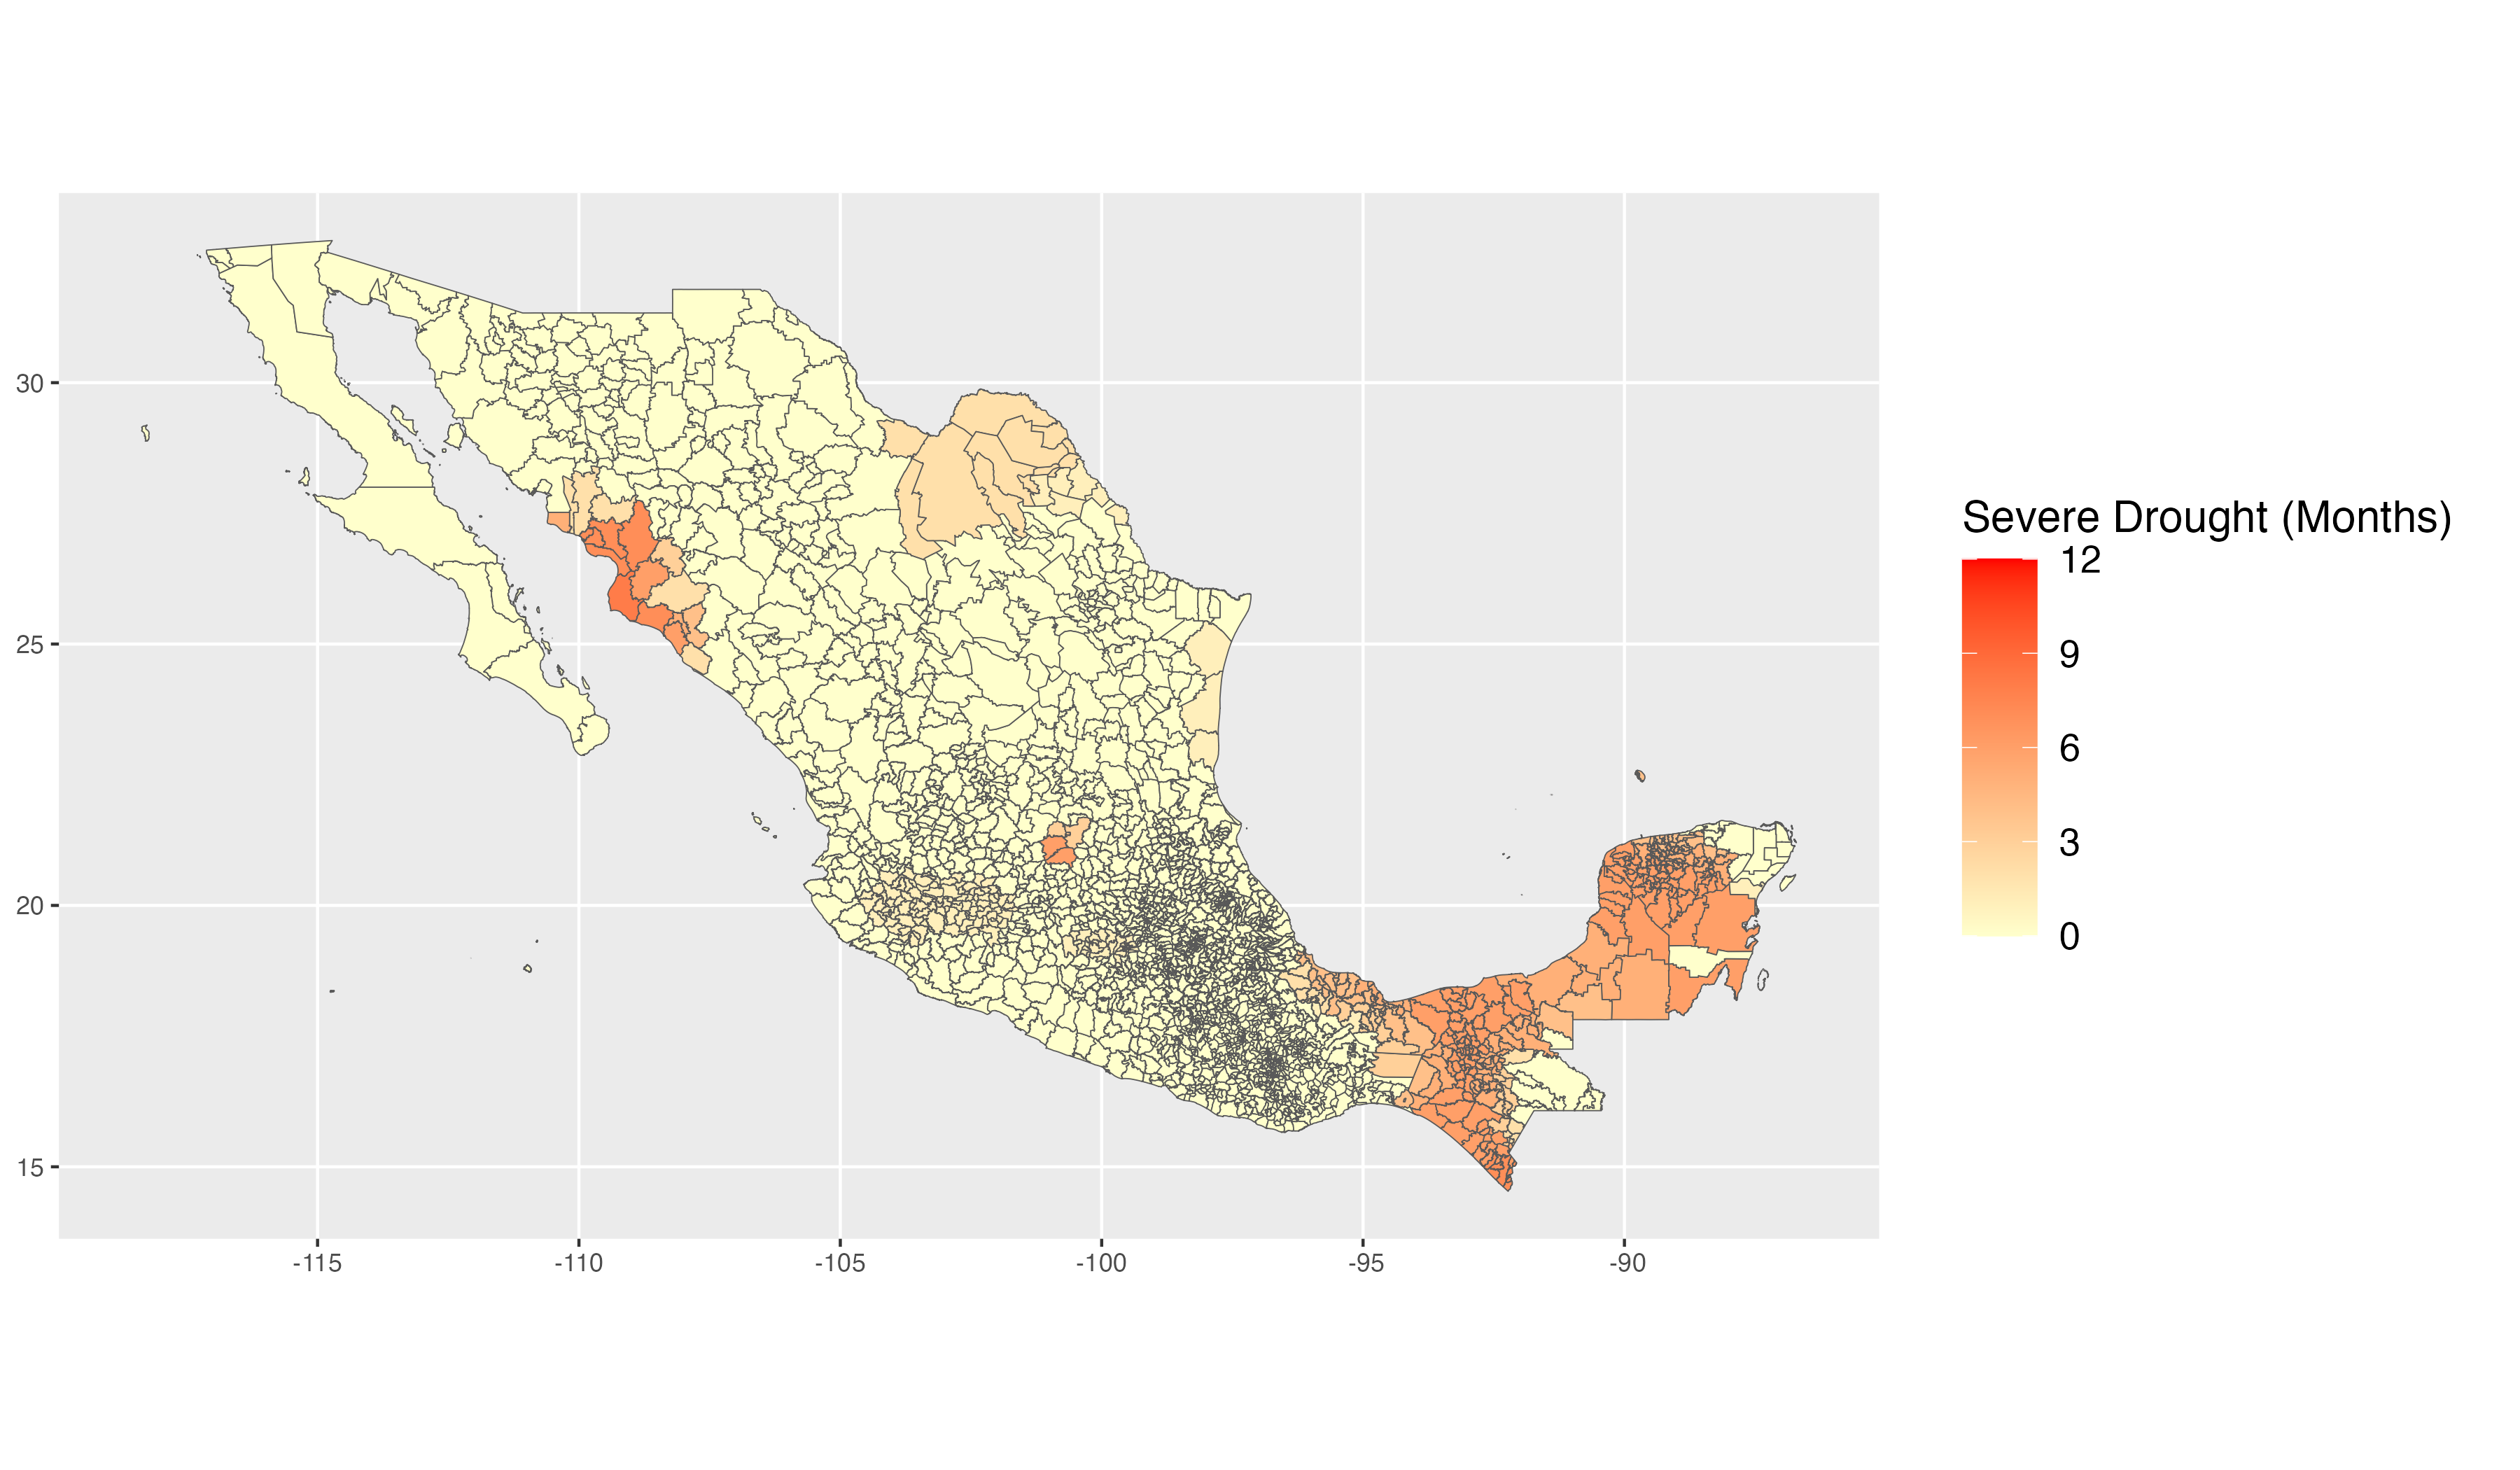
\includegraphics[width=\linewidth]{figures/drought_2010.png} % Update the file name as needed
        \caption*{Panel a) 2010}
    \end{minipage}
    \hfill % this will insert a little space between your minipages
    % Second minipage
    \begin{minipage}[b]{0.55\textwidth}
        \centering
        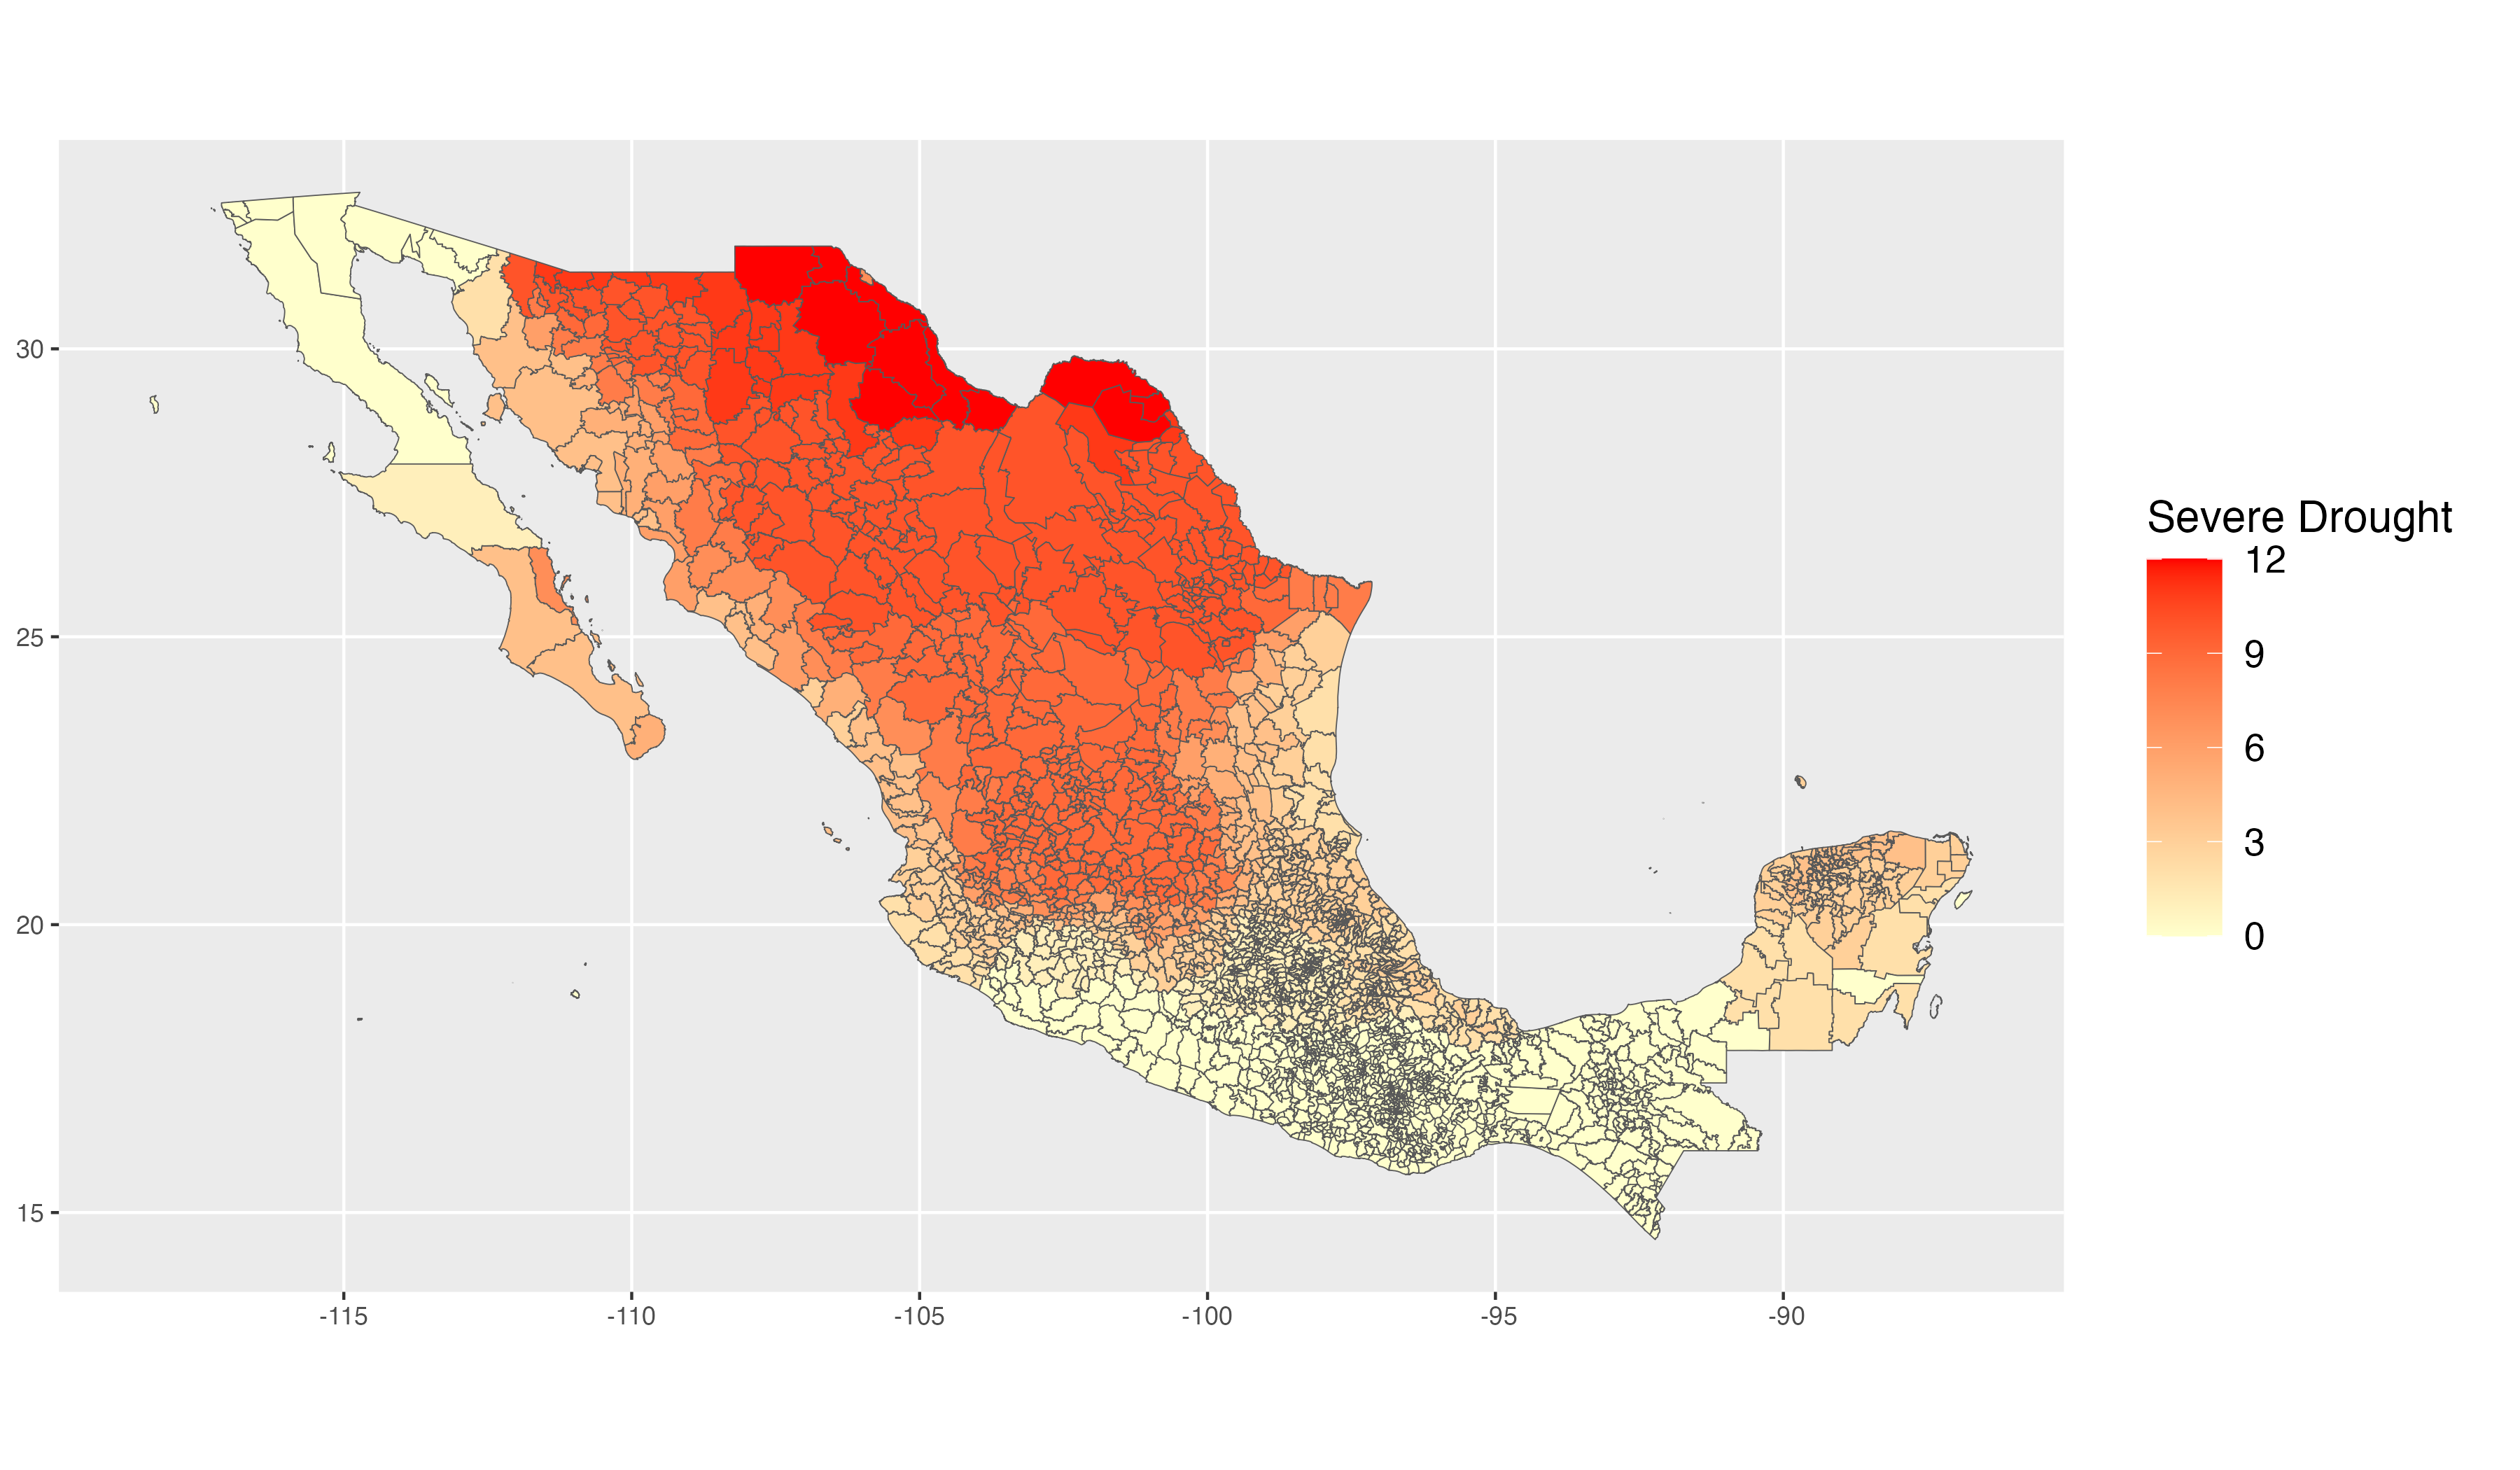
\includegraphics[width=\linewidth]{figures/drought_2011.png} % Update the file name as needed
        \caption*{Panel b) 2011}
    \end{minipage}
    \hfill
    % Third minipage
    \begin{minipage}[b]{0.55\textwidth}
        \centering
        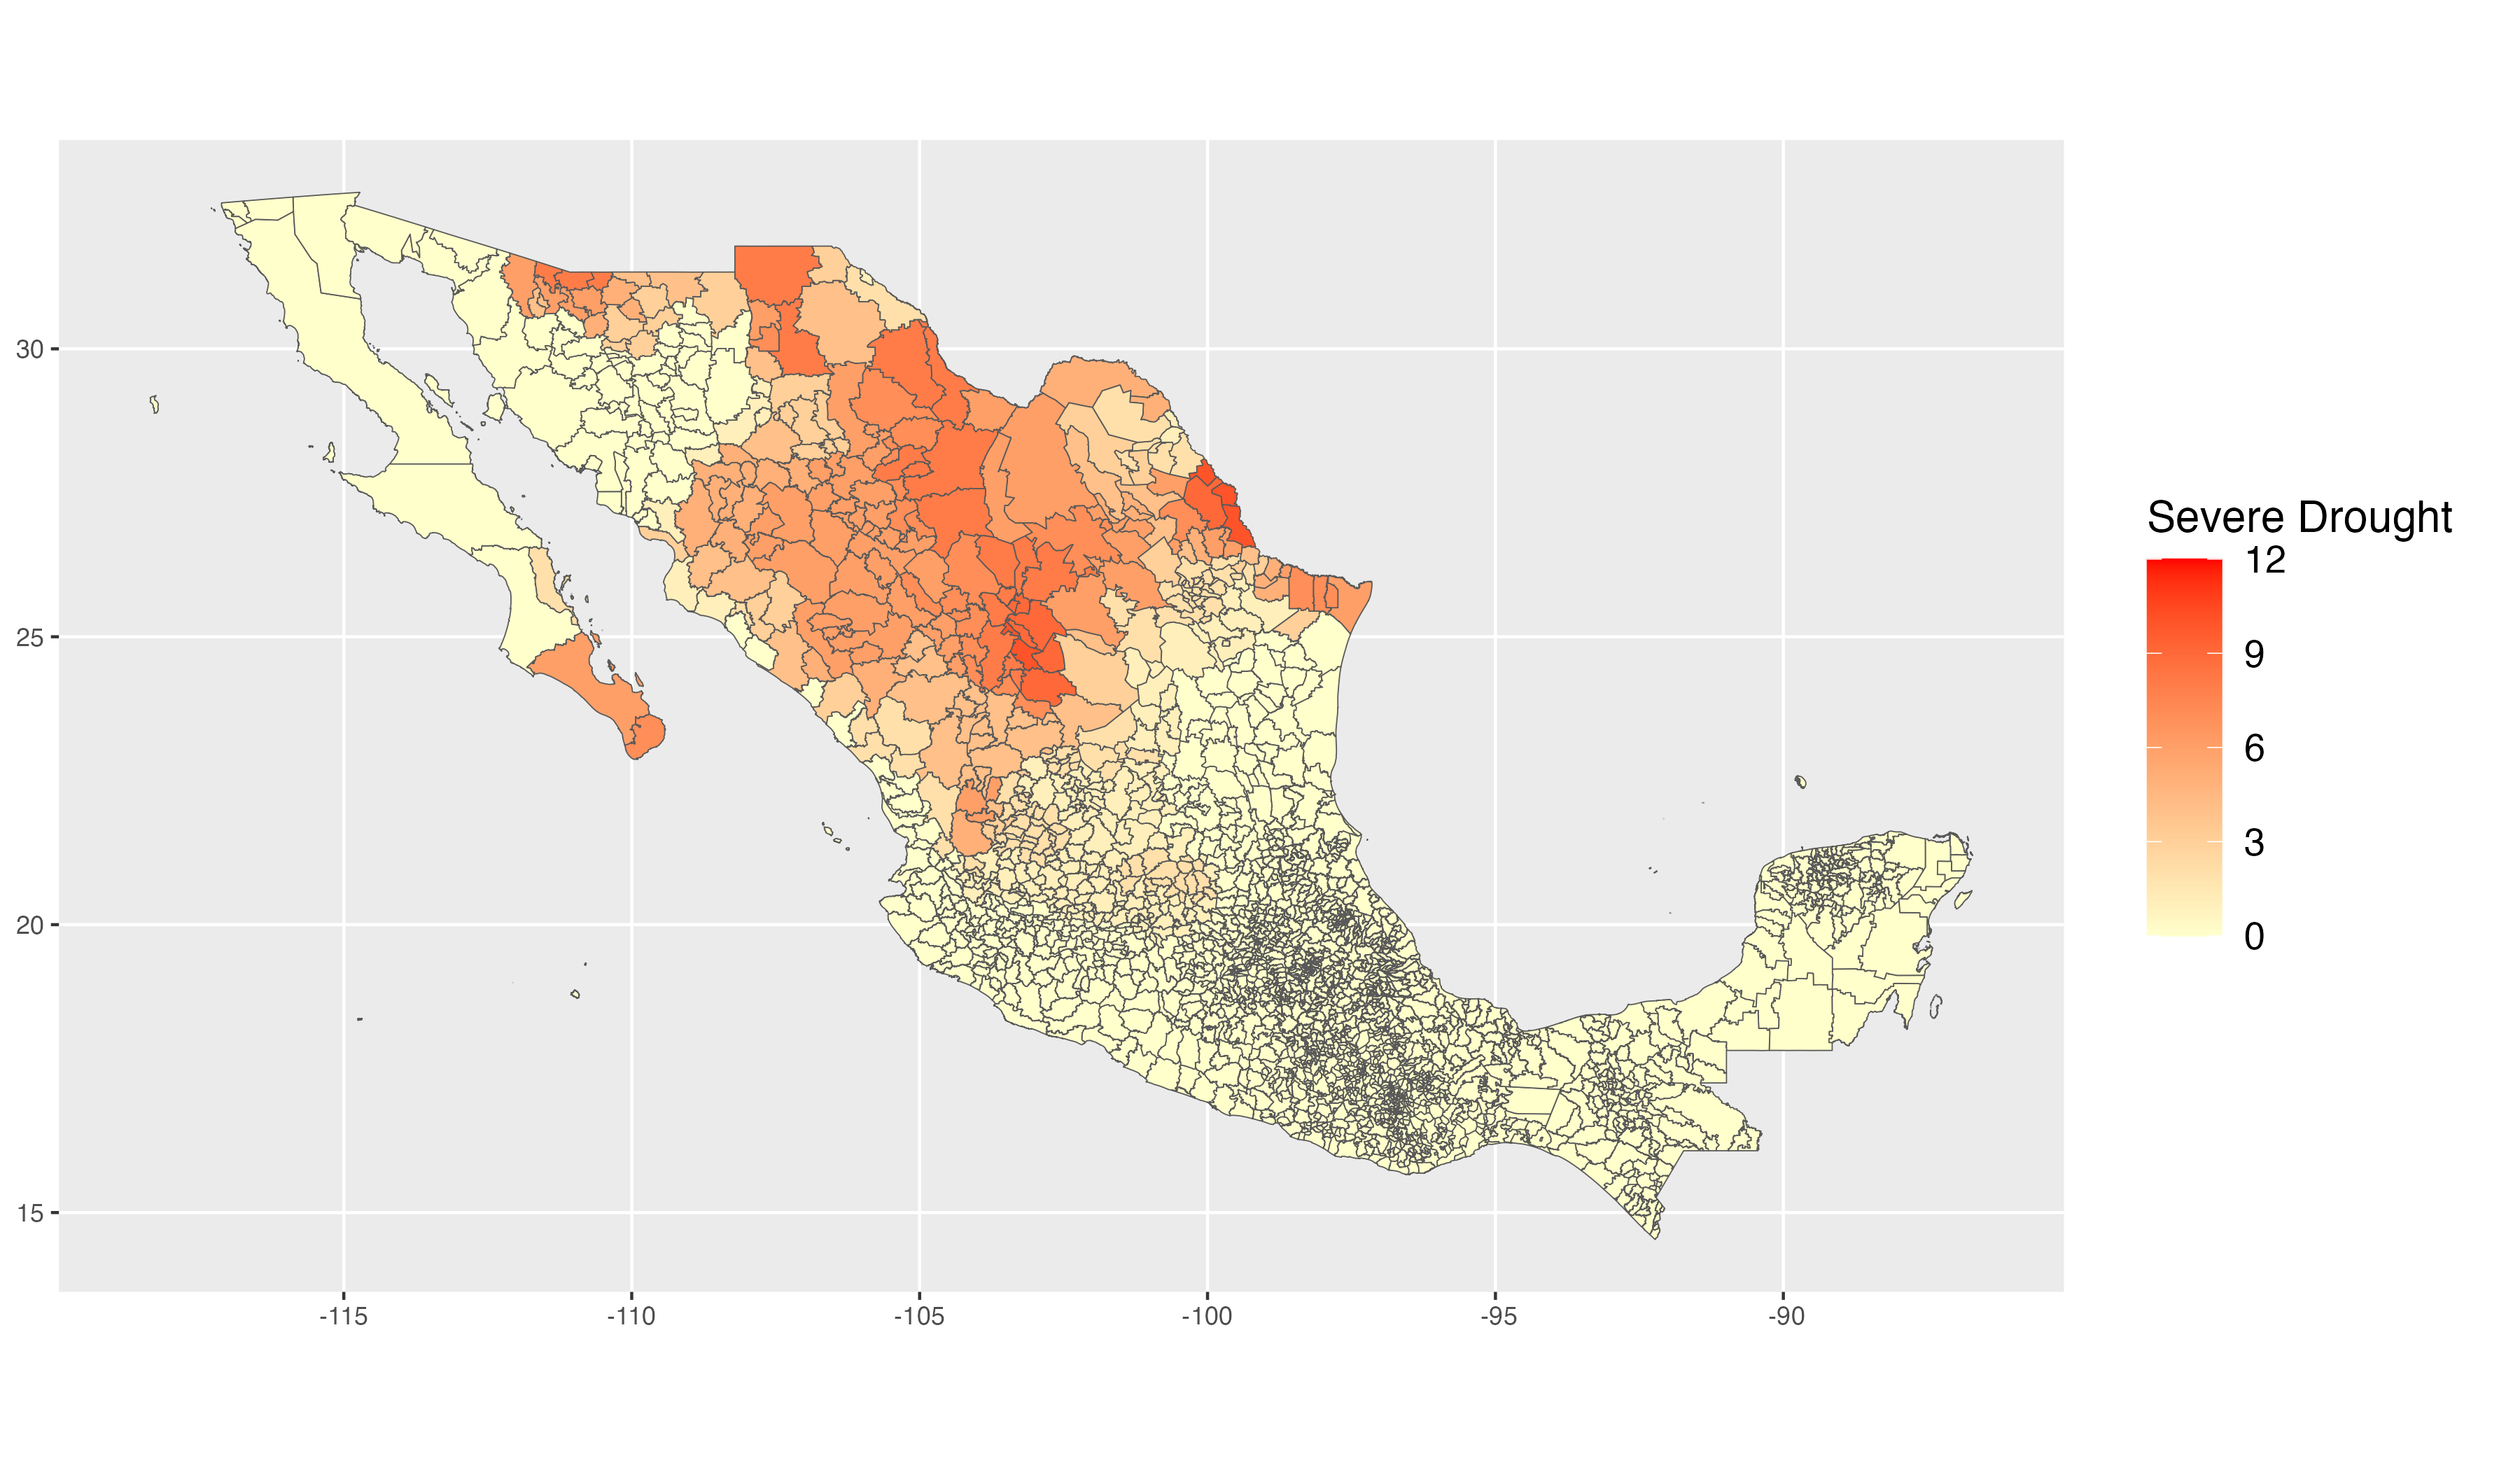
\includegraphics[width=\linewidth]{figures/drought_2012.png} % Update the file name as needed
        \caption*{Panel c) 2012}
    \end{minipage}
    \label{fig:droughts_geographical}
    \caption*{\footnotesize{Notes: Most intense red color reflects 12 months with drought registries in D2, D3, or D4. Yellow color reflects 0 registries of drought of those categories}}
\end{figure}



\clearpage
\newpage

\begin{table}[!ht]
\begin{center}
\caption{Descriptive Statistics. Drought categories}\label{tab:descriptives_drought}
\resizebox{\textwidth}{!}{%
\begin{tabular}{lccccc}  
\toprule

\textbf{Panel A. Birth outcomes} &&& && \\

                    &\multicolumn{1}{c}{No drought}&\multicolumn{1}{c}{D0}&\multicolumn{1}{c}{D1}&\multicolumn{1}{c}{D2}&\multicolumn{1}{c}{D3-D4}\\\cmidrule(lr){2-2}\cmidrule(lr){3-3}\cmidrule(lr){4-4}\cmidrule(lr){5-5}\cmidrule(lr){6-6}
                    &\multicolumn{1}{c}{}&\multicolumn{1}{c}{}&\multicolumn{1}{c}{}&\multicolumn{1}{c}{}&\multicolumn{1}{c}{}\\
\midrule
Weight at birth     &    3,155.04&    3,161.87&    3,170.06&    3,183.30&    3,206.57\\
                    &    (199.38)&    (198.63)&    (186.26)&    (179.80)&    (194.57)\\
Weight at birth     &       49.94&       49.97&       50.02&       50.10&       50.24\\
                    &      (1.10)&      (1.10)&      (1.05)&      (1.02)&      (1.13)\\
APGAR               &        8.84&        8.84&        8.85&        8.84&        8.86\\
                    &      (0.46)&      (0.45)&      (0.38)&      (0.43)&      (0.42)\\
Silverman           &        0.20&        0.22&        0.21&        0.22&        0.23\\
                    &      (0.46)&      (0.49)&      (0.43)&      (0.43)&      (0.61)\\
Total consultations &        7.08&        7.06&        7.00&        6.96&        7.07\\
                    &      (1.46)&      (1.40)&      (1.32)&      (1.23)&      (1.36)\\
Any prenatal care   &       79.13&       78.51&       76.34&       74.74&       74.61\\
                    &     (41.18)&     (39.43)&     (32.72)&     (29.36)&     (30.84)\\
Low birth weight    &        4.05&        4.11&        3.93&        3.87&        3.92\\
                    &     (10.16)&      (8.90)&      (8.97)&      (6.66)&      (8.24)\\
Very low borth weight&        0.39&        0.42&        0.41&        0.41&        0.46\\
                    &      (2.93)&      (2.81)&      (2.98)&      (2.30)&      (3.75)\\
Preterm             &        4.74&        4.84&        4.79&        4.93&        5.19\\
                    &     (10.52)&      (9.20)&      (9.74)&      (7.99)&      (9.47)\\
Macrosomia          &        1.72&        1.88&        1.91&        2.03&        2.37\\
                    &      (6.92)&      (5.81)&      (6.19)&      (4.67)&      (5.91)\\
Congenital Anomaly  &        2.37&        2.55&        2.39&        2.30&        2.82\\
                    &      (8.70)&      (9.59)&      (8.79)&      (7.84)&      (9.06)\\
APGAR < 7           &        1.15&        1.13&        1.10&        1.21&        1.10\\
                    &      (6.33)&      (6.00)&      (5.60)&      (4.32)&      (4.47)\\
\midrule
Observations        &     200,020&      74,682&      37,282&      14,528&       6,403\\
 \\

\textbf{Panel B. Newborn and mother's hospitalizations} &&& && \\
\\
\midrule
Total hosp.         &       65.69&       70.84&       72.73&       66.80&       66.33\\
                    &    (156.91)&    (155.95)&    (147.36)&    (124.64)&    (135.66)\\
Neonatal comp       &       40.36&       44.70&       46.59&       42.72&       39.56\\
                    &    (121.59)&    (120.41)&    (117.04)&     (97.79)&    (100.52)\\
Respiratory         &        8.80&        8.75&        8.36&        8.52&       12.01\\
                    &     (46.14)&     (60.38)&     (35.05)&     (29.76)&     (56.71)\\
Digestive           &        1.31&        1.23&        1.29&        1.27&        1.61\\
                    &     (21.42)&     (20.26)&     (12.44)&     (12.19)&     (18.28)\\
Other infections    &        2.15&        2.39&        2.37&        2.52&        2.99\\
                    &     (19.50)&     (24.97)&     (20.55)&     (21.69)&     (23.04)\\
External            &        0.75&        0.72&        0.66&        0.59&        0.68\\
                    &     (13.63)&     (11.43)&      (7.11)&      (5.33)&      (5.92)\\
Pregnancy complications&      266.43&      261.75&      263.82&      260.35&      230.21\\
                    &    (337.21)&    (329.33)&    (324.76)&    (255.63)&    (245.37)\\
\midrule
Observations        &     183,201&      63,987&      27,119&      10,758&       5,752\\
 \\

\bottomrule
\end{tabular}}
\noindent
\caption*{\footnotesize{Notes:  }}
\end{center}
\end{table}

\clearpage
\newpage




\section{Methods}

I closely follow the methodology used in previous research \cite{Bailey2015}, \cite{Mullins2020}, \cite{Cohen2022} to explore the effects of weather conditions, specifically the impact of drought intensity on pregnancy, births, and newborn health outcomes. Drought intensity is measured using CONAGUA's monthly Drought Monitor index whose scale ranges from abnormally dry (D0) to exceptional drought (D4). Categories D3-D4 are pooled together to ensure enough variation in the higher end of drought.

Using CONAGUA's monthly Drought Monitor index, this empirical strategy captures nonlinear effects on outcomes by exploiting drought categorizations from the preceding month to explain current outcomes. Drought effects often accumulate and are not immediately apparent, as droughts typically intensify or recede gradually. Health outcomes, such as those related to water scarcity or air quality, may take time to manifest. Therefore, a 1-month lag drought measure could better capture the delayed effects on current health outcomes, aligning with the gradual onset and impact of droughts.\footnote{I also use current month drought measures, but these soesnt change the estimates by much. I present these results in the Appendix}

Specifically, I consider a fixed-effects linear regression model of the form:

\begin{align}
\begin{aligned}
Y_{imy} &= \beta_0 + \sum_{k=1}^{3/4} \beta_k D^k_{i(m-1)y} + \phi_1 \cdot Temp_{imy} + \lambda_i + \lambda_{my} + \epsilon_{im}
\end{aligned}
\label{eq:temp_regression}
\end{align}

where $Y_{imy}$ is the outcome in municipality $i$ in month $m$ and year $y$. $\sum_{k=0}^{3/4} \beta_k D_{ki(m-1)y}$ captures the effects of drought intensity across categories $D^0$ to $D^{3/4}$, measured in the previous month. The model includes municipality-specific fixed effects ($\lambda_i$) to account for time-invariant characteristics, month-by-year fixed effects ($\lambda_{my}$) for unobserved factors affecting monthly outcomes across municipalities, and municipality-year fixed effects ($\lambda_{iy}$) to account for differential trends over years.


The key identifying assumption is that, conditional on the fixed effects and temperatures, the remaining variation from drought intensity is exogenous and uncorrelated with other factors influencing health and birth outcomes. This assumption is widely accepted and used in the literature mentioned in the introduction.


\section{Results. Impact of Drought on Health}


\subsection{During pregnancy}

We would expect that current temperature has a significant effect on pregnancy outcomes, as extreme environmental conditions during critical periods can impose immediate physiological stress on both the mother and the fetus. Extreme temperatures and drought conditions can induce thermal stress, affecting cardiovascular and thermoregulatory systems, leading to complications such as preterm labor. Additionally, unusual dry conditions can cause dehydration, reduce amniotic fluid, and increase the risk of preterm birth. It can also raise blood pressure, increasing the risk of preeclampsia. Acute weather changes can lead to hospital admissions for both mothers and newborns, as heatwaves may increase existing conditions (\cite{Ha2022}, \cite{Kim2021}).

Figure \ref{fig:effects_pregnancy_drought} panel a) presents the impact of different drought categories on the hospitalization rates of pregnant women, excluding those related to regular deliveries. We can observe that the rate of hospitalizations due to pregnancy complications increases with exposure to more intense drought categories, while the number of consultations shows a seemingly parabolic decreasing trend. In both outcomes, the category corresponding to the most intense drought exposure (D3-D4) has the greatest magnitudes and statistically significant effects.

It is important to note that the timing of exposure differs between these outcomes. For hospitalizations, drought exposure is measured 1 month before the hospitalization occurs, while for prenatal care and total consultations, the exposure is measured 1 month before birth, as this information is recorded at that time. (I have to check this specification as it might make more sense to track the exposure during all the pregnancy rather than 1 month before birth)

Table \ref{tab:effects_mothers_drought} provides a detailed breakdown of the magnitudes of these coefficients and includes a variable that measures the rate of cases in which mothers had at least one checkup during their entire pregnancy. As a robustness check, the second column of each subgroup also incorporates municipality-by-calendar-month fixed effects, following the approach of \cite{Cohen2022}, to account for seasonal variations that recur annually within municipalities.

The results in Table \ref{tab:effects_mothers} show that mothers' hospitalizations increase as drought severity rises, with coefficients for D2 (17.96) and D3-D4 (17.65) indicating a significant increase in pregnancy-related hospital admissions per 1,000 births. \footnote{Specifications using the log of the number of hospitalizations, instead of the rate, were also tested. The results are qualitatively similar and are presented in the Appendix.} This pattern suggests that more intense droughts are linked to higher rates of pregnancy complications, as reported in previous research. On the other hand, prenatal care appears largely unaffected, except for the more severe drought categories, with minimal changes in the share of women receiving at least one check-up. Total consultations, show a gradual decline as drought severity increases, especially for D3-D4. This could reflect barriers to accessing care or shifts in healthcare-seeking behavior during extreme drought periods.

In terms of magnitudes, the increase in hospitalizations for severe droughts (D3-D4) translates to about 17 additional hospitalizations per 1,000 births monthly, which is substantial. Meanwhile, the reduction in total consultations, while smaller, indicates a drop of approximately 0.048 consultations per 1,000 births. While not all coefficients are statistically significant, the general escalation in hospitalization rates with more intense droughts aligns with what we would expect given the potential health risks posed by such environmental stressors.


\begin{figure}[!ht]
    \centering
    \caption{Effects during pregnancy}
    \begin{minipage}[b]{0.6\textwidth}
        \centering
        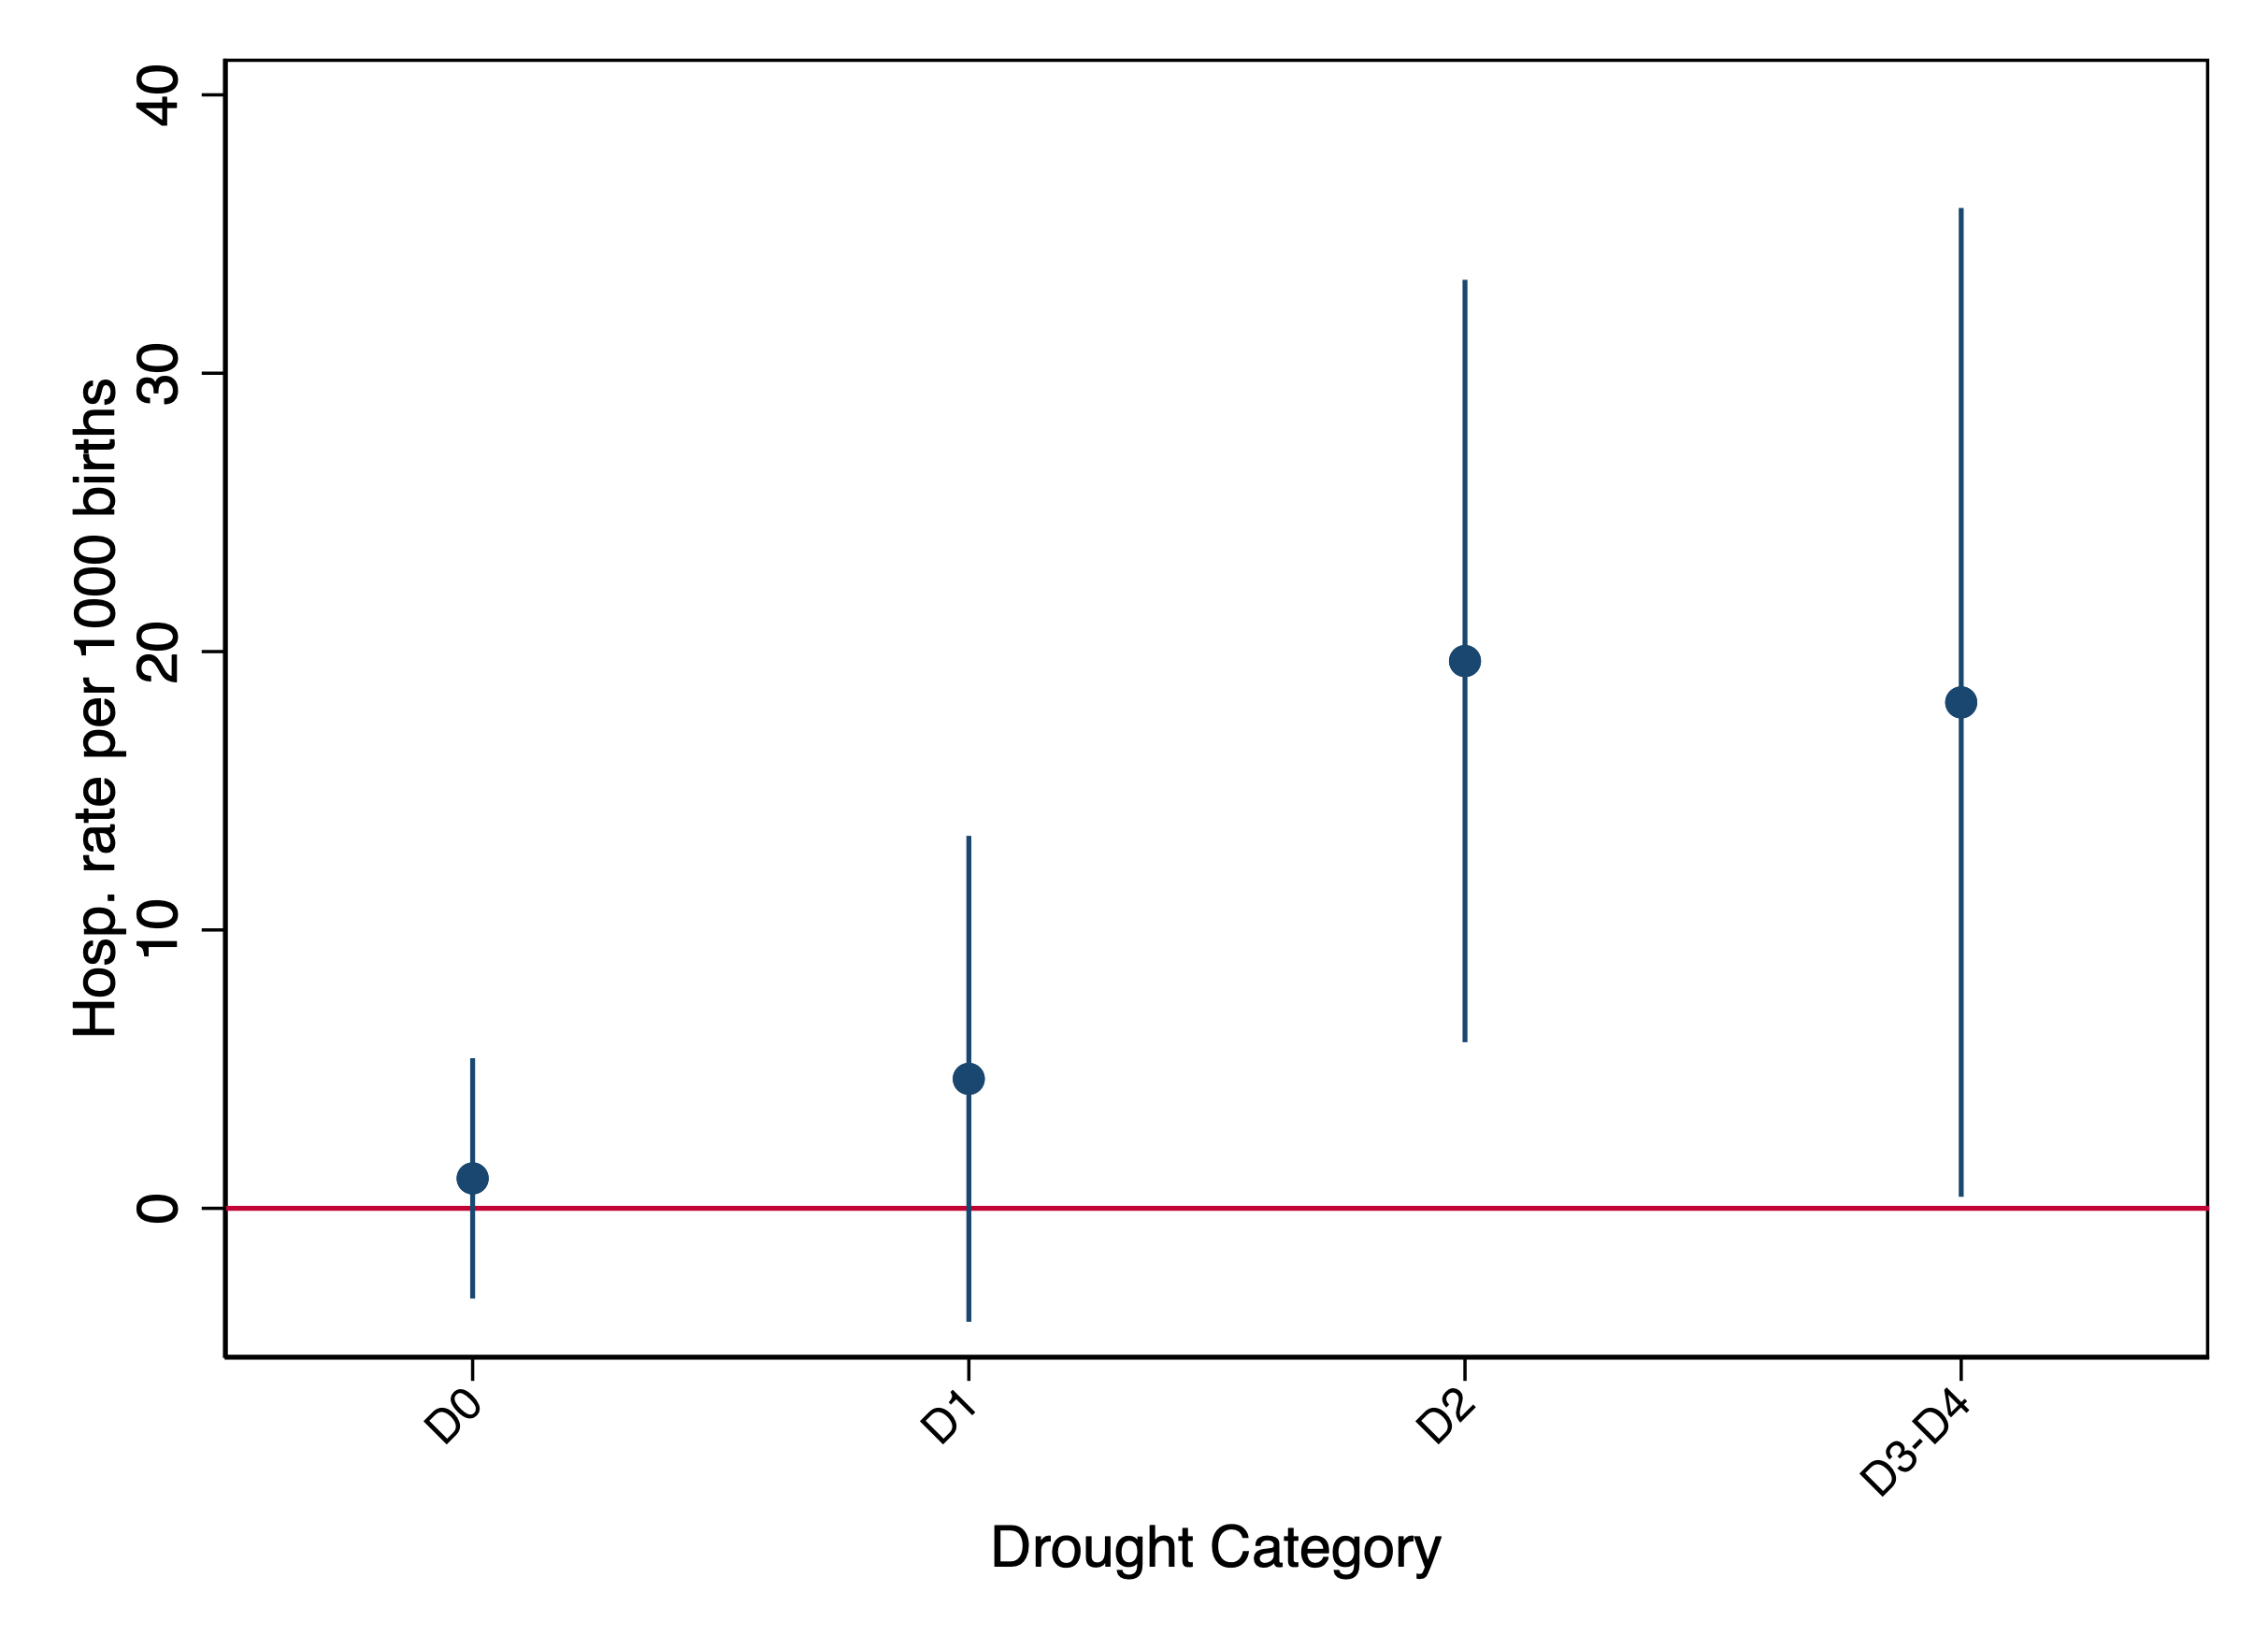
\includegraphics[width=\linewidth]{figures_2410/02_maternal_muni_by_Dcategory.png} % Update the file name as needed
     \caption*{Panel a) Hospitalizations}
    \end{minipage}
    \begin{minipage}[b]{0.6\textwidth}
        \centering
        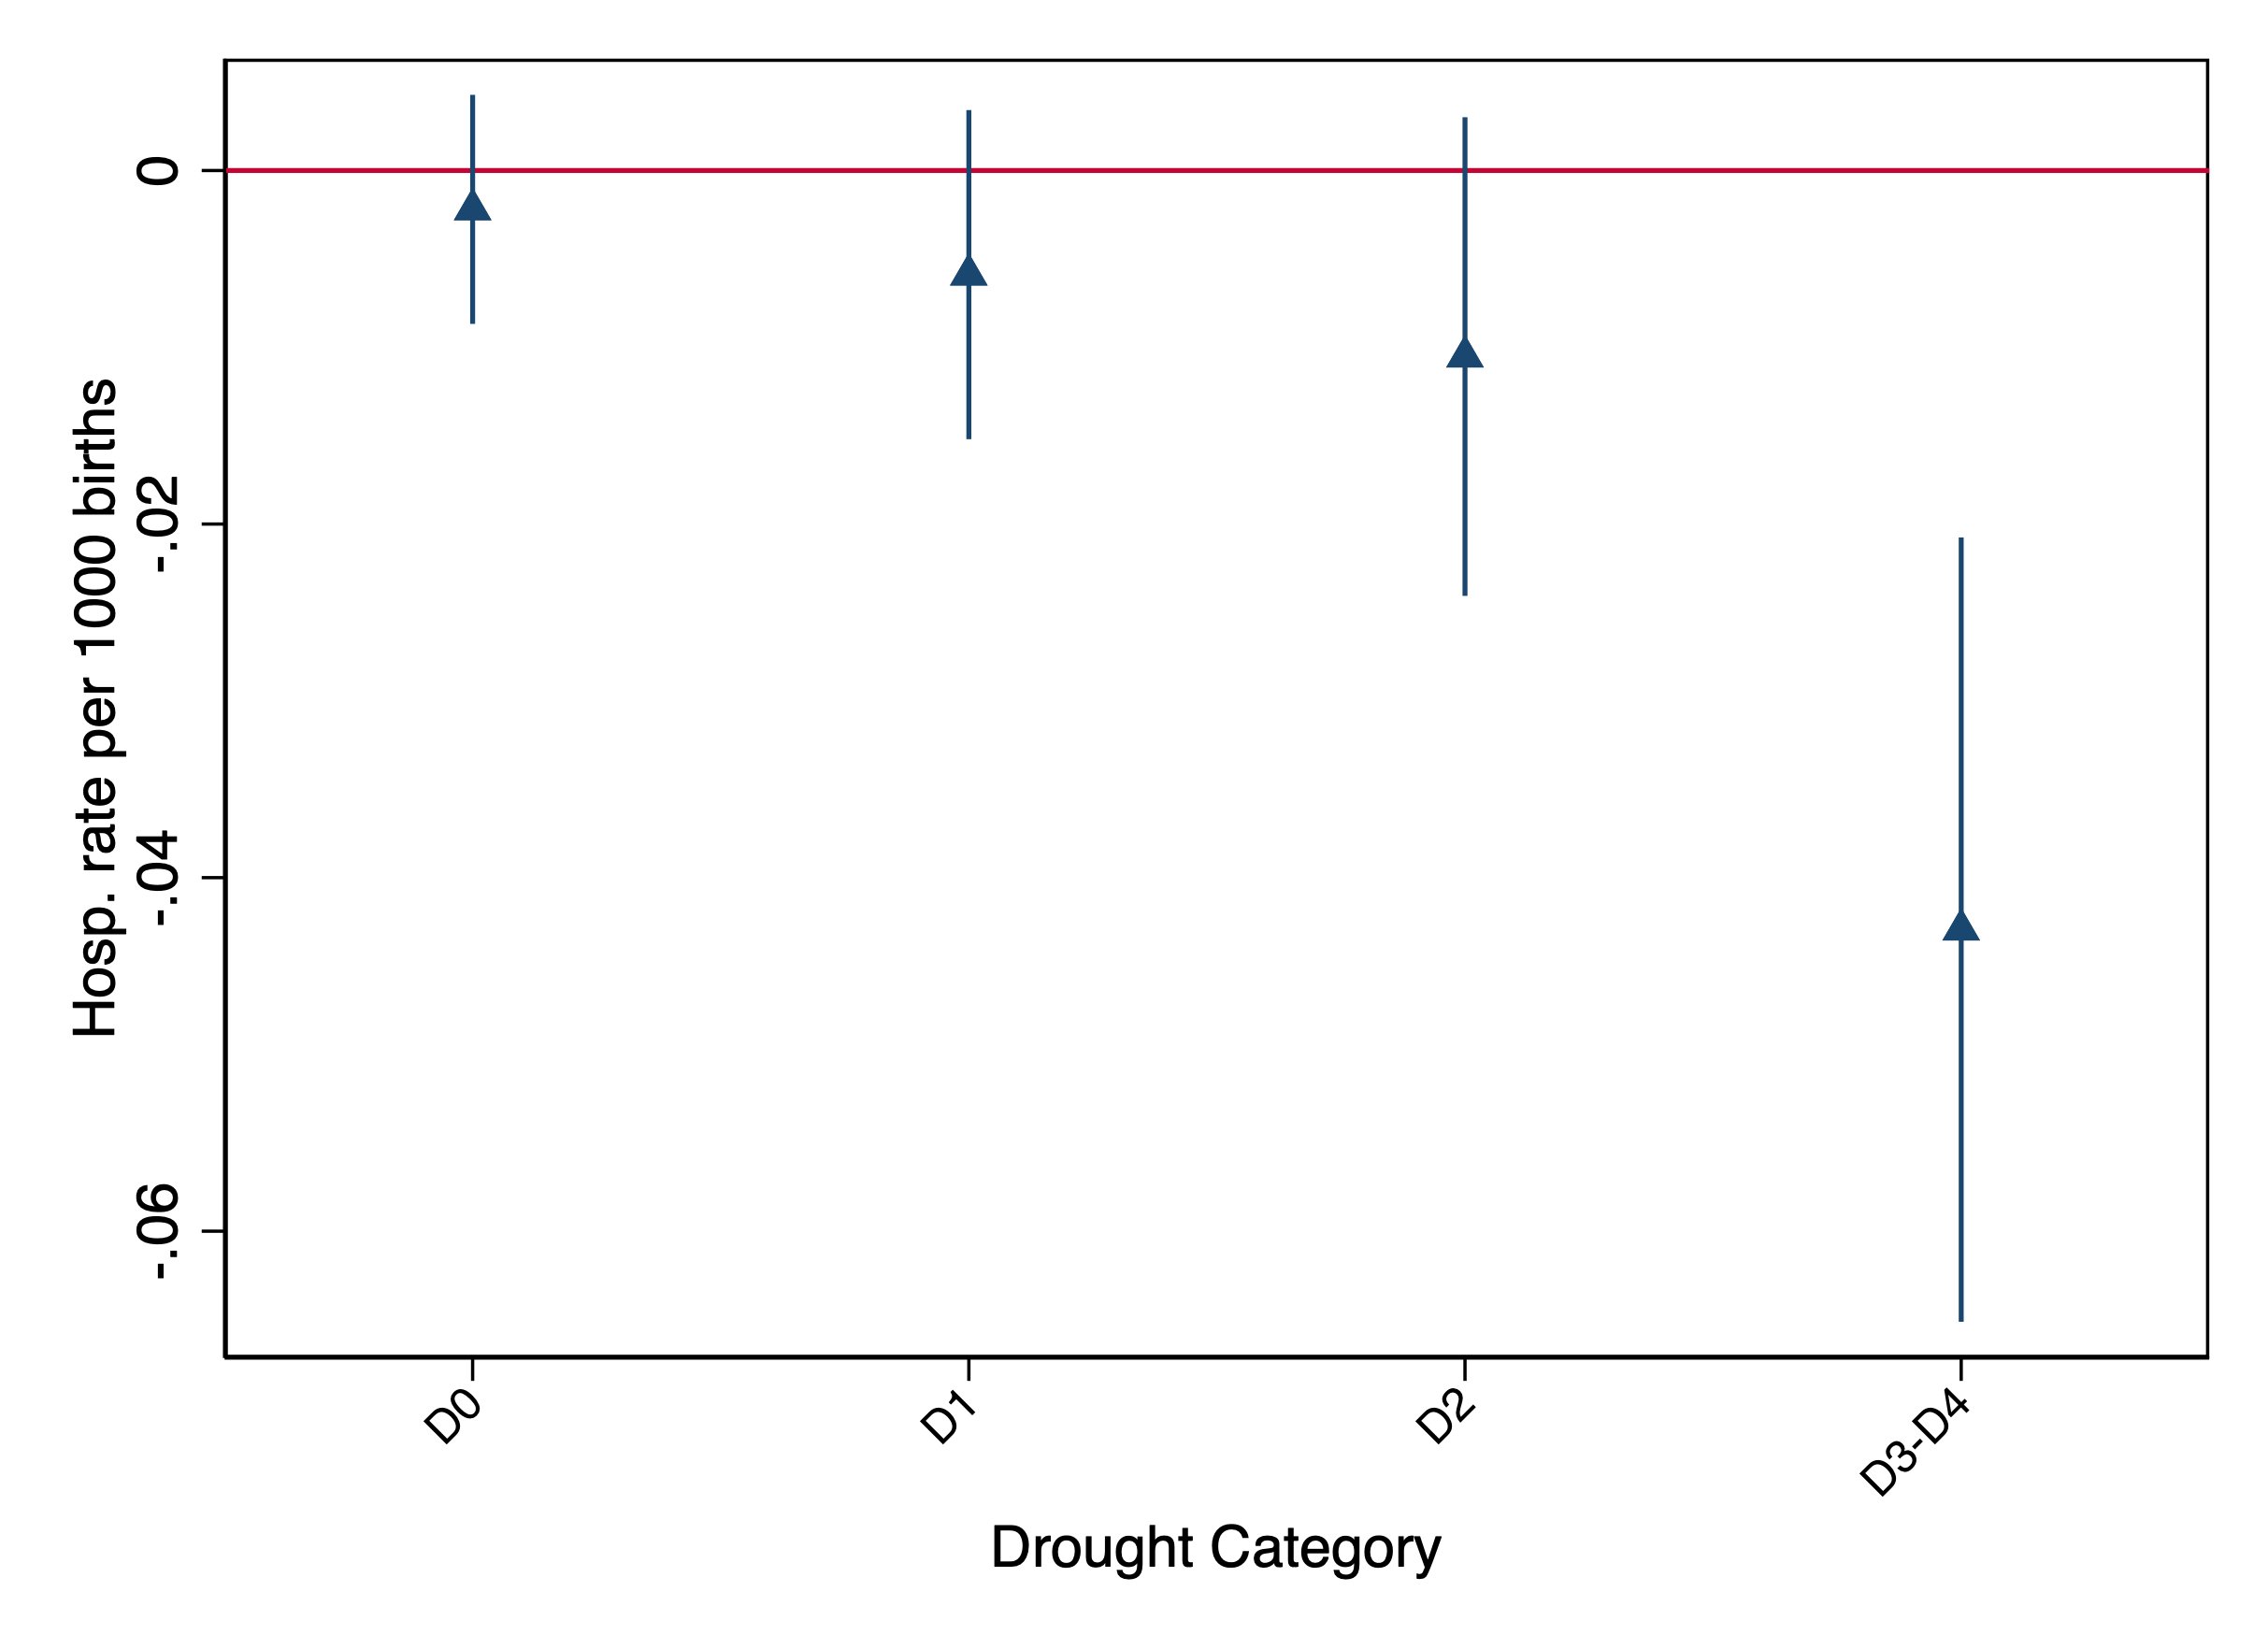
\includegraphics[width=\linewidth]{figures_2410/02_total_consult_muni_by_Dcategory.png} % Update the file name as needed
 \caption*{Panel b) Number of consultations }
    \end{minipage}
    \label{fig:effects_pregnancy_drought}
    \caption*{\footnotesize{Notes: Panel a) shows the effect of drought intensity on the hospitalizations rate of women due to pregnancy complications per 1000 births. Drought intensity is measured using CONAGUA's monthly Drought Monitor index whose scale ranges from abnormally dry (D0) to exceptional drought (D4).Categories D3-D4 are pooled together to ensure enough variation in the higher end of drought. Pregnancy complications are defined according to the ICD-10 codes O00-O9A corresponding to Pregnancy, childbirth and the puerperium. Codes O80, O81, and O82 are omitted because they correspond to regular labor and delivery. This measure comes from the SSA discharges database. Panel b) present the results for the total number of consultations or checkups during pregnancy.This variable comes from the birth certificates (SINAC) database. Standard errors are clustered at the municipality-calendar month level.}}
\end{figure}

\clearpage
\newpage

\begin{table}[!ht]
\centering
\caption{Effects of drought during pregnancy}\label{tab:effects_mothers_drought}
\fontsize{10pt}{12pt}\selectfont
\begin{tabularx}{\textwidth}{Xcccccc}
\toprule
&\multicolumn{2}{c}{Hospitalizations} &\multicolumn{2}{c}{Any prenatal care} &\multicolumn{2}{c}{Total consultations} \\
\cmidrule(lr){2-3}\cmidrule(lr){4-5}\cmidrule(lr){6-7}

\midrule
D0                  &       0.099   &      -0.266   &      -0.000   &      -0.000   &      -0.002   &      -0.003   \\
                    &     (2.387)   &     (2.541)   &     (0.000)   &     (0.000)   &     (0.003)   &     (0.003)   \\
D1                  &       3.976   &       1.261   &      -0.000   &      -0.000   &      -0.005   &      -0.004   \\
                    &     (3.965)   &     (4.137)   &     (0.000)   &     (0.000)   &     (0.005)   &     (0.005)   \\
D2                  &      17.960***&      15.596** &      -0.001   &      -0.001   &      -0.011   &      -0.016** \\
                    &     (6.409)   &     (6.751)   &     (0.000)   &     (0.000)   &     (0.007)   &     (0.007)   \\
D3-D4               &      17.649** &      13.831*  &      -0.003***&      -0.003***&      -0.042***&      -0.048***\\
                    &     (8.022)   &     (8.292)   &     (0.001)   &     (0.001)   &     (0.011)   &     (0.012)   \\
\midrule
Observations        &     236,220   &     235,752   &     288,174   &     287,969   &     288,174   &     287,969   \\
Mean Y              &      381.81   &      381.81   &        0.98   &        0.98   &        7.35   &        7.35   \\
Month-year            &     \(\times\)   &      \(\times\)   &    \(\times\)    &    \(\times\)  &   \(\times\)   &  \(\times\) \\
Municipality-year           &     \(\times\)   &      \(\times\)   &    \(\times\)    &    \(\times\)  &   \(\times\)   &  \(\times\) \\
Municipality-calendar month             &       &      \(\times\)   &       &    \(\times\)  &     &  \(\times\) \\
 \\

\bottomrule
\end{tabularx}
\caption*{\footnotesize{Notes: This table summarizes the effects of drought intensity, as measured using CONAGUA's monthly Drought Monitor index whose scale ranges from abnormally dry (D0) to exceptional drought (D4) on maternal health outcomes. Categories D3-D4 are pooled together to ensure enough variation in the higher end of drought. Hospitalizations are measured as the rate of monthly hospitalizations during pregnancy per 1000 births. Pregnancy complications are defined according to the ICD-10 codes O00-O9A corresponding to Pregnancy, childbirth and the puerperium. Codes O80, O81, and O82 are omitted because they correspond to regular labor and delivery admissions. This measure comes from the SSA discharges database. Any prenatal care is measured as the share of mothers who had at least one consultation or check-up during pregnancy in certain municipality. Total consultations is the average number of consultations during pregnancy within a municipality. These last two variables come from the birth certificates (SINAC) database. All regressions control for current and 1 month lagged temperatures. Standard errors are clustered at the municipality-calendar month level. $^* p<0.1, ^{**} p<0.05, ^{***} p<0.01$.}}
\end{table}


\subsection{At birth}

Table \ref{tab:results_at_birth_drought} present results for several birth outcomes. Panel A present point estimates of the main specification that includes the three sets of fixed effects discussed in the methods section, while Panel B includes the municipality-by-month seasonal effects suggested in \cite{Cohen2022} as a robustness check.

The results indicate that drought severity has a cumulative impact on birth outcomes, consistent with medical literature on environmental stress. Although not all coefficients are statistically significant, there is an increasing trend in the estimates for more severe drought categories. Very Low Birth Weight (VLBW) is consistently significant, with larger magnitudes in moderate drought (D1, D2), suggesting that drought-induced maternal stress likely compromises fetal development. This aligns with broader research linking maternal stress to poor birth outcomes, particularly under nutritional or environmental pressure (\cite{Ha2022}, \cite{Meherali2024}). Though the estimates for Low Birth Weight (LBW) and Preterm births are not significant, their positive directions reflect previous established risks related to preterm labor under environmental stress \cite{Jain2021}.

C-section and congenital anomalies show statistically significant effects only under the most severe drought conditions (D3-D4). The rise in C-section rates under extreme drought (6.16 in Panel B) may reflect heightened medical interventions due to fetal distress, consistent with obstetric literature that ties severe maternal stress and environmental hardship to higher-risk deliveries. Similarly, the large increase in congenital anomalies (5.118***) for extreme droughts supports findings from environmental health research linking exposure to heat, pollution, and malnutrition during pregnancy to birth defects \cite{Ha2022}.

To put these results in context, it is helpful to compare the coefficient estimates to the means of the respective outcomes. For VLBW, the increase of 0.770 under moderate drought conditions (D2) represents a 16\% rise relative to the mean of 4.78, suggesting a considerable impact on the likelihood of very low birth weight. For C-sections, the increase of 6.16 under severe drought (D3-D4) corresponds to a modest 1.5\% rise from the mean of 401.54, indicating a smaller, though still meaningful, effect. The most striking result is for congenital anomalies, where the marginal effect of 5.118 under severe drought reflects an 18.5\% rise from the mean of 27.69.


\begin{table}[!ht]
\begin{center}
\caption{Effects of drought on birth outcomes}\label{tab:results_at_birth_drought}
\fontsize{10pt}{12pt}\selectfont
\begin{tabularx}{\textwidth}{Xcccccc}
\toprule

\textbf{Panel A. Base Model} & & & & & \\
  &\multicolumn{1}{c}{LBW}&\multicolumn{1}{c}{VLBW}&\multicolumn{1}{c}{Preterm}&\multicolumn{1}{c}{C-section}&\multicolumn{1}{c}{Anomaly} \\\cmidrule(lr){2-2}\cmidrule(lr){3-3}\cmidrule(lr){4-4}\cmidrule(lr){5-5}\cmidrule(lr){6-6}
\midrule
D0                  &       0.288   &       0.291*  &      -0.581   &      -0.649   &      -0.268   \\
                    &     (0.479)   &     (0.154)   &     (0.523)   &     (1.069)   &     (0.386)   \\
D1                  &       0.318   &       0.512** &      -0.643   &       2.631*  &       0.096   \\
                    &     (0.703)   &     (0.254)   &     (0.764)   &     (1.549)   &     (0.577)   \\
D2                  &       0.898   &       0.770** &       0.041   &       3.060   &       0.225   \\
                    &     (0.985)   &     (0.388)   &     (1.118)   &     (2.187)   &     (0.810)   \\
D3-D4               &       0.688   &       0.722   &       1.360   &       8.961** &       5.356***\\
                    &     (1.550)   &     (0.476)   &     (1.723)   &     (3.479)   &     (1.436)   \\
\midrule
Observations        &     288,791   &     288,791   &     288,791   &     288,791   &     288,791   \\
Mean Y              &       48.25   &        4.78   &       57.71   &      401.54   &       27.69   \\
 \\
\midrule
\textbf{Panel B. Base Model + Seasonal FE} & & & & & \\
D0                  &       0.387   &       0.297*  &      -0.406   &      -0.694   &      -0.212   \\
                    &     (0.499)   &     (0.161)   &     (0.547)   &     (1.109)   &     (0.402)   \\
D1                  &       0.261   &       0.436*  &      -0.837   &       1.394   &      -0.017   \\
                    &     (0.730)   &     (0.253)   &     (0.800)   &     (1.599)   &     (0.587)   \\
D2                  &       0.694   &       0.732*  &      -0.305   &       0.792   &       0.207   \\
                    &     (1.021)   &     (0.404)   &     (1.157)   &     (2.266)   &     (0.824)   \\
D3-D4               &      -0.370   &       0.640   &       0.210   &       6.160*  &       5.118***\\
                    &     (1.621)   &     (0.498)   &     (1.790)   &     (3.587)   &     (1.421)   \\
\midrule
Observations        &     288,596   &     288,596   &     288,596   &     288,596   &     288,596   \\
Mean Y              &       48.25   &        4.78   &       57.71   &      401.54   &       27.69   \\
 \\

\bottomrule
\end{tabularx}
\noindent
\caption*{\footnotesize{This table summarizes the effects of drought intensity on birth outcomes. Drought intensity is measured using CONAGUA's monthly Drought Monitor index, which ranges from abnormally dry (D0) to exceptional drought (D4). Categories D3-D4 are pooled to ensure sufficient variation at the higher end of the drought scale. Birth weight is measured in grams, with Low Birth Weight (LBW) defined as less than 2,500 grams and Very Low Birth Weight (VLBW) as less than 1,500 grams. Preterm refers to births occurring at less than 37 weeks of gestation. C-section is the monthly rate of cesarean deliveries per 1,000 births, and Anomaly refers to the rate of congenital malformations, coded Q00-Q99 according to ICD-10. Standard errors are clustered at the municipality-calendar month level. $^* p<0.1, ^{**} p<0.05, ^{***} p<0.01$.}}
\end{center}
\end{table}

\clearpage
\newpage

\subsection{Newborn health}



\clearpage
\newpage


\begin{table}[!ht]
\centering
\caption{Effects of Drought on Newborn Health}\label{tab:hospital_drought}
\fontsize{10pt}{12pt}\selectfont
\begin{tabular}{lccccc}
\toprule
\textbf{Panel A. Base Model} & & & & & \\
                    &\multicolumn{1}{c}{Total hosp.}&\multicolumn{1}{c}{Neonatal comp}&\multicolumn{1}{c}{Respiratory}&\multicolumn{1}{c}{Digestive}&\multicolumn{1}{c}{External}\\\cmidrule(lr){2-2}\cmidrule(lr){3-3}\cmidrule(lr){4-4}\cmidrule(lr){5-5}\cmidrule(lr){6-6}
\midrule
D0                  &       0.457   &       0.142   &       0.081   &      -0.019   &      -0.069   \\
                    &     (1.340)   &     (1.056)   &     (0.357)   &     (0.130)   &     (0.092)   \\
D1                  &       1.755   &       0.175   &      -0.768   &       0.528** &       0.041   \\
                    &     (1.864)   &     (1.401)   &     (0.550)   &     (0.230)   &     (0.167)   \\
D2                  &       3.681   &       0.972   &      -1.087   &       0.329   &      -0.191   \\
                    &     (2.328)   &     (1.693)   &     (0.782)   &     (0.277)   &     (0.221)   \\
D3-D4               &       0.697   &       0.796   &      -0.004   &       0.421   &      -0.148   \\
                    &     (3.135)   &     (2.246)   &     (1.252)   &     (0.455)   &     (0.298)   \\
\midrule
Observations        &     260,147   &     260,147   &     260,147   &     260,147   &     260,147   \\
Mean Y              &      100.01   &       62.25   &       12.91   &        1.86   &        1.07   \\
 \\

\textbf{Panel B. Base Model + Seasonal FE} & & & & & \\
D0                  &       1.454   &       0.965   &       0.042   &      -0.005   &      -0.080   \\
                    &     (1.391)   &     (1.080)   &     (0.370)   &     (0.137)   &     (0.098)   \\
D1                  &       3.020   &       1.397   &      -0.475   &       0.495** &       0.060   \\
                    &     (2.006)   &     (1.523)   &     (0.554)   &     (0.229)   &     (0.175)   \\
D2                  &       5.040** &       2.244   &      -0.765   &       0.342   &      -0.098   \\
                    &     (2.517)   &     (1.851)   &     (0.817)   &     (0.282)   &     (0.222)   \\
D3-D4               &       2.064   &       2.220   &       0.197   &       0.486   &      -0.095   \\
                    &     (3.360)   &     (2.359)   &     (1.299)   &     (0.463)   &     (0.322)   \\
\midrule
Observations        &     259,861   &     259,861   &     259,861   &     259,861   &     259,861   \\
Mean Y              &      100.01   &       62.25   &       12.91   &        1.86   &        1.07   \\
 \\
\bottomrule
\end{tabular}
\caption*{\footnotesize{Notes: This table summarizes the effects of of drought intensity on newborn health outcomes. Drought intensity is measured using CONAGUA's monthly Drought Monitor index whose scale ranges from abnormally dry (D0) to exceptional drought (D4).Categories D3-D4 are pooled together to ensure enough variation in the higher end of drought. Hospitalizations are measured as the rate of hospitalizations during pregnancy per 1000 births.  Hospitalizations due to specific causes are identified using ICD-10 codes. Respiratory causes include conditions such as bronchitis and pneumonia (codes starting with "J"), digestive causes include intestinal infectious diseases (codes A00-A09), neonatal complications and congenital malformations are indicated by "P" or "Q," and external causes include injuries and accidents (codes "T," "S," "V," "W," "X," or "Y"). These measures comes from the SSA discharges database. Standard errors are clustered at the municipality-calendar month level. $^* p<0.1, ^{**} p<0.05, ^{***} p<0.01$.}}
\end{table}


\clearpage
\newpage



\section{The effect of Progresa and Seguro Popular}

To investigate the potential shock-absorbing capacity of Progresa and Seguro Popular, I use a method similar to \cite{Barreca2016} and \cite{Cohen2022}. Specifically, I interact the availability of Progresa in each municipality, as measured by the proportion of beneficiary households in each municipality and year, with the indicators of drought intensity. It is important to note that the proportion of Progresa beneficiaries increased slightly year by year, reflecting the expansion in coverage up to 2019 (the year in which Progresa was rolled back).

Because Progresa primarily targets low-income families, the coefficient for the main effect of Progresa cannot be interpreted as causal. Nevertheless, since drought intensity provides exogenous variation, conditional on all fixed effects and covariates, interactions between Progresa and each drought category inform us about the mitigating effect of this conditional cash transfer program on weather vulnerability.

Additionally, I include a set of interactions between each drought category and month-by-year fixed effects to control for the autonomous evolution of weather conditions that are unrelated to the evolution of Progresa's expansion.          


\subsection{During pregnancy}

\begin{table}[!ht]
\centering
\caption{Effects of Drought on Pregnancy}\label{tab:hospital_drought}
\fontsize{10pt}{12pt}\selectfont
\begin{tabular}{lcccccc}
\toprule
\textbf{Panel A. Progresa} & & & & & & \\
                    &\multicolumn{2}{c}{Mother hospit.}&\multicolumn{2}{c}{Total consultations}&\multicolumn{2}{c}{Any prenatal care}                          \\\cmidrule(lr){2-3}\cmidrule(lr){4-5}\cmidrule(lr){6-7}
\midrule
D0                  &       3.659   &       5.817   &      -0.012   &       0.000   &      -0.001   &      -0.000   \\
                    &     (7.756)   &     (7.844)   &     (0.013)   &     (0.013)   &     (0.001)   &     (0.001)   \\
D1                  &       4.230   &       3.577   &      -0.017   &       0.009   &      -0.001   &      -0.001   \\
                    &    (13.989)   &    (14.173)   &     (0.018)   &     (0.019)   &     (0.001)   &     (0.001)   \\
D2                  &       4.746   &       4.435   &       0.022   &       0.042   &      -0.001   &      -0.000   \\
                    &    (19.646)   &    (19.969)   &     (0.026)   &     (0.026)   &     (0.002)   &     (0.002)   \\
D3-D4               &     -27.002   &     -31.431   &       0.096** &       0.129***&       0.009***&       0.005*  \\
                    &    (25.553)   &    (26.443)   &     (0.045)   &     (0.043)   &     (0.003)   &     (0.002)   \\
\midrule
Observations        &     203,895   &     203,880   &     280,053   &     280,036   &     280,053   &     280,036   \\
Mean Y              &      381.31   &      381.31   &        7.35   &        7.35   &        0.98   &        0.98   \\
 \\
\midrule
\textbf{Panel B. Seguro Popular} & & & & & & \\
D0                  &      -1.079   &       0.538   &      -0.020   &      -0.005   &       0.000   &       0.000   \\
                    &     (9.723)   &     (9.766)   &     (0.013)   &     (0.014)   &     (0.001)   &     (0.001)   \\
D1                  &     -11.800   &     -12.814   &      -0.020   &       0.017   &       0.001   &       0.001   \\
                    &    (15.173)   &    (15.089)   &     (0.018)   &     (0.020)   &     (0.001)   &     (0.001)   \\
D2                  &     -13.839   &     -10.280   &       0.012   &       0.034   &       0.001   &       0.001   \\
                    &    (23.975)   &    (25.254)   &     (0.027)   &     (0.029)   &     (0.002)   &     (0.002)   \\
D3-D4               &      20.472   &      28.261   &       0.104** &       0.137***&       0.010***&       0.007***\\
                    &    (39.445)   &    (40.100)   &     (0.046)   &     (0.047)   &     (0.003)   &     (0.002)   \\
\midrule
Observations        &     203,895   &     203,880   &     280,053   &     280,036   &     280,053   &     280,036   \\
Mean Y              &      381.31   &      381.31   &        7.35   &        7.35   &        0.98   &        0.98   \\
Municipality-calendar month             &   \(\times\)    &      \(\times\)   &    \(\times\)   &    \(\times\)  & \(\times\)    &  \(\times\) \\
Month-year $\times$  Drought         &      &      \(\times\)   &       &    \(\times\)  &   &  \(\times\)  \\
\bottomrule
\end{tabular}
\caption*{\footnotesize{Notes: All specifications include municipality FE, municipality-year FE, month-year FE, municipality-by-calendar month FE. $^* p<0.1, ^{**} p<0.05, ^{***} p<0.01$.}}
\end{table}


\subsection{At birth}




\subsection{Newborn health after birth}

\begin{table}[!ht]
\centering
\caption{Effects of Drought on Newborn Health}\label{tab:hospital_drought}
\fontsize{10pt}{12pt}\selectfont
\begin{tabular}{lcccccc}
\toprule
\textbf{Panel A. Progresa} & & & &  \\
                    &\multicolumn{2}{c}{Total hosp.}&\multicolumn{1}{c}{Neonatal comp} \\\cmidrule(lr){2-3}\cmidrule(lr){4-5}
\midrule
D0                  &       5.861   &       5.281   &       4.580*  &       4.504   \\
                    &     (4.196)   &     (4.259)   &     (2.778)   &     (2.807)   \\
D1                  &      -2.433   &      -4.369   &      -1.942   &      -2.355   \\
                    &     (6.388)   &     (6.463)   &     (4.563)   &     (4.740)   \\
D2                  &      -0.997   &      -6.037   &      -1.524   &      -1.870   \\
                    &     (7.875)   &     (7.980)   &     (5.461)   &     (5.502)   \\
D3-D4               &     -25.563** &     -28.240** &      -9.557   &      -9.442   \\
                    &    (11.897)   &    (11.857)   &     (7.842)   &     (8.430)   \\
\midrule
Observations        &     225,087   &     225,071   &     225,087   &     225,071   \\
Mean Y              &       99.90   &       99.90   &       62.17   &       62.17   \\
 \\
\midrule
\textbf{Panel B. Seguro Popular} & & & & \\

D0                  &       0.225   &      -0.662   &       1.734   &       1.734   \\
                    &     (4.624)   &     (4.652)   &     (3.459)   &     (3.502)   \\
D1                  &     -21.152***&     -23.990***&      -9.297*  &      -9.614*  \\
                    &     (6.925)   &     (7.001)   &     (4.993)   &     (5.021)   \\
D2                  &       1.492   &      -3.049   &       6.673   &       6.439   \\
                    &    (10.033)   &    (10.319)   &     (6.859)   &     (7.087)   \\
D3-D4               &     -18.788   &     -20.434   &       1.096   &       1.432   \\
                    &    (12.352)   &    (13.001)   &     (8.838)   &     (9.292)   \\
\midrule
Observations        &     225,087   &     225,071   &     225,087   &     225,071   \\
Mean Y              &       99.90   &       99.90   &       62.17   &       62.17   \\
 \\
\bottomrule
\end{tabular}
\caption*{\footnotesize{Notes: All specifications include municipality FE, municipality-year FE, month-year FE, municipality-by-calendar month FE. $^* p<0.1, ^{**} p<0.05, ^{***} p<0.01$.}}
\end{table}

\clearpage
\newpage


\section{Heterogeneity in the effect of Progresa and Seguro Popular}

\begin{table}[!ht]
\centering
\caption{Program Heterogeneity. Mother's outcomes}\label{tab:program_heterogeneity_mothers}
\fontsize{10pt}{12pt}\selectfont
\begin{tabular}{lcccccc}
\toprule
\textbf{Panel A. Progresa} & & & &  \\
                    &\multicolumn{2}{c}{Mother hospit.}&\multicolumn{2}{c}{Total consultations}&\multicolumn{2}{c}{Any prenatal care}                          \\\cmidrule(lr){2-3}\cmidrule(lr){4-5}\cmidrule(lr){6-7}
                    
&\multicolumn{1}{c}{HP}&\multicolumn{1}{c}{LP}&\multicolumn{1}{c}{HP}&\multicolumn{1}{c}{LP}&\multicolumn{1}{c}{HP}&\multicolumn{1}{c}{LP} \\
                    
\midrule
D0                  &      53.734** &      -4.896   &      -0.038   &      -0.002   &      -0.000   &      -0.000   \\
                    &    (23.343)   &    (13.085)   &     (0.054)   &     (0.016)   &     (0.005)   &     (0.001)   \\
D1                  &      39.862   &     -14.196   &      -0.108   &       0.015   &      -0.010   &      -0.000   \\
                    &    (44.006)   &    (18.565)   &     (0.087)   &     (0.023)   &     (0.007)   &     (0.001)   \\
D2                  &      75.604   &      -3.301   &      -0.058   &       0.037   &      -0.015   &       0.000   \\
                    &    (79.813)   &    (30.620)   &     (0.133)   &     (0.032)   &     (0.010)   &     (0.002)   \\
D3-D4               &      43.257   &     -54.834   &       0.100   &       0.115** &      -0.013   &       0.008***\\
                    &    (92.090)   &    (37.888)   &     (0.239)   &     (0.052)   &     (0.022)   &     (0.002)   \\
\midrule
Observations        &      54,888   &     148,973   &      54,448   &     225,561   &      54,448   &     225,561   \\
Mean Y              &      395.94   &      375.46   &        6.15   &        7.42   &        0.96   &        0.98   \\
 \\
\midrule
\textbf{Panel B. Seguro Popular} & & & & \\
\\

\midrule
D0                  &      44.099   &      -7.741   &      -0.039   &      -0.007   &      -0.001   &       0.001   \\
                    &    (35.674)   &    (12.056)   &     (0.078)   &     (0.015)   &     (0.006)   &     (0.001)   \\
D1                  &     -49.745   &     -14.751   &       0.078   &       0.015   &       0.003   &       0.001   \\
                    &    (56.993)   &    (17.141)   &     (0.113)   &     (0.022)   &     (0.009)   &     (0.001)   \\
D2                  &    -130.095   &      -3.409   &       0.300   &       0.026   &       0.002   &       0.001   \\
                    &    (87.594)   &    (30.611)   &     (0.208)   &     (0.031)   &     (0.013)   &     (0.002)   \\
D3-D4               &    -225.440*  &      45.690   &      -0.273   &       0.128** &      -0.007   &       0.008***\\
                    &   (128.979)   &    (47.279)   &     (0.281)   &     (0.050)   &     (0.019)   &     (0.002)   \\
\midrule
Observations        &      54,888   &     148,973   &      54,448   &     225,561   &      54,448   &     225,561   \\
Mean Y              &      395.94   &      375.46   &        6.15   &        7.42   &        0.96   &        0.98   \\
 \\
\bottomrule
\end{tabular}
\caption*{\footnotesize{Notes: All specifications include municipality FE, municipality-year FE, month-year FE, municipality-by-calendar month FE. $^* p<0.1, ^{**} p<0.05, ^{***} p<0.01$.}}
\end{table}

\clearpage
\newpage


\begin{table}[!ht]
\centering
\caption{Program Heterogeneity. Birth outcomes}\label{tab:program_heterogeneity_birth}
\fontsize{10pt}{12pt}\selectfont
\begin{tabular}{lcccccc}
\toprule
\textbf{Panel A. Progresa} & & & &  \\
                    &\multicolumn{2}{c}{VLBW}&\multicolumn{2}{c}{Anomaly}&\multicolumn{2}{c}{C-section} \\\cmidrule(lr){2-3}\cmidrule(lr){4-5}\cmidrule(lr){6-7}
&\multicolumn{1}{c}{HP}&\multicolumn{1}{c}{LP}&\multicolumn{1}{c}{HP}&\multicolumn{1}{c}{LP}&\multicolumn{1}{c}{HP}&\multicolumn{1}{c}{LP} \\
\midrule
D0                  &       3.134*  &      -1.496   &       1.695   &       2.610   &       3.509   &      -2.941   \\
                    &     (1.614)   &     (1.049)   &     (4.055)   &     (2.545)   &    (12.344)   &     (6.933)   \\
D1                  &       2.120   &       1.395   &      -7.098   &       2.078   &     -23.123   &       3.802   \\
                    &     (3.082)   &     (1.472)   &     (6.497)   &     (3.435)   &    (17.469)   &     (9.671)   \\
D2                  &      -2.809   &      -3.585*  &     -16.467*  &      -2.809   &      14.198   &     -11.068   \\
                    &     (4.060)   &     (1.901)   &     (9.520)   &     (4.281)   &    (25.463)   &    (12.589)   \\
D3-D4               &      -4.897   &      -2.207   &     -29.007*  &       2.951   &     -38.177   &      -6.002   \\
                    &     (7.334)   &     (2.561)   &    (16.958)   &     (7.854)   &    (48.567)   &    (20.186)   \\
\midrule
Observations        &      75,255   &     205,353   &      75,255   &     205,353   &      75,255   &     205,353   \\
Mean Y              &        3.91   &        5.11   &       22.53   &       29.63   &      297.20   &      440.79   \\
 \\
\midrule
\textbf{Panel B. Seguro Popular} & & & & \\
   \\
\midrule
D0                  &       2.754   &      -1.335   &       1.165   &      -2.090   &      42.664** &     -11.273*  \\
                    &     (2.348)   &     (0.951)   &     (5.202)   &     (2.459)   &    (17.897)   &     (6.475)   \\
D1                  &       5.709   &       0.660   &      -8.686   &      -1.560   &      13.029   &       3.353   \\
                    &     (3.603)   &     (1.231)   &     (7.298)   &     (3.156)   &    (23.748)   &     (8.641)   \\
D2                  &      -1.352   &      -3.945*  &      -1.758   &      -0.771   &      19.825   &     -11.621   \\
                    &     (5.575)   &     (2.280)   &    (11.225)   &     (4.076)   &    (35.699)   &    (12.341)   \\
D3-D4               &       2.044   &      -3.127   &       0.555   &       2.743   &     -32.192   &     -46.631** \\
                    &     (7.183)   &     (2.614)   &    (21.981)   &     (7.041)   &    (68.224)   &    (18.371)   \\
\midrule
Observations        &      75,255   &     205,353   &      75,255   &     205,353   &      75,255   &     205,353   \\
Mean Y              &        3.91   &        5.11   &       22.53   &       29.63   &      297.20   &      440.79   \\
 \\
\bottomrule
\end{tabular}
\caption*{\footnotesize{Notes: All specifications include municipality FE, municipality-year FE, month-year FE, municipality-by-calendar month FE. $^* p<0.1, ^{**} p<0.05, ^{***} p<0.01$.}}
\end{table}



\clearpage
\newpage

\begin{table}[!ht]
\centering
\caption{Program Heterogeneity. Babies' hospitalizations}\label{tab:program_heterogeneity_babies}
\fontsize{10pt}{12pt}\selectfont
\begin{tabular}{lcccc}
\toprule
\textbf{Panel A. Progresa} & &   \\
                    &\multicolumn{2}{c}{Total hosp.}&\multicolumn{2}{c}{Neonatal comp.}\\\cmidrule(lr){2-3}\cmidrule(lr){4-5}

&\multicolumn{1}{c}{HP}&\multicolumn{1}{c}{LP}&\multicolumn{1}{c}{HP}&\multicolumn{1}{c}{LP} \\
\midrule
D0                  &      10.953   &      11.106*  &      13.651   &       0.104   \\
                    &    (13.828)   &     (6.572)   &     (8.866)   &     (4.357)   \\
D1                  &      10.395   &     -19.523** &       8.603   &      -8.664   \\
                    &    (20.018)   &     (9.019)   &    (15.260)   &     (6.664)   \\
D2                  &     -33.602   &     -19.579*  &     -33.907*  &     -12.786*  \\
                    &    (26.083)   &    (11.808)   &    (19.981)   &     (7.513)   \\
D3-D4               &     -45.309   &     -37.363** &     -11.561   &     -23.801** \\
                    &    (41.939)   &    (17.549)   &    (28.144)   &    (12.047)   \\
\midrule
Observations        &      60,851   &     164,198   &      60,851   &     164,198   \\
Mean Y              &      113.70   &       94.66   &       71.24   &       58.73   \\
 \\
\midrule
\textbf{Panel B. Seguro Popular} & &  \\
\\
                    
\midrule
D0                  &       2.860   &      -0.848   &       2.417   &      -1.618   \\
                    &    (16.044)   &     (5.598)   &    (12.598)   &     (4.257)   \\
D1                  &     -52.763** &     -29.452***&     -23.392   &     -11.076*  \\
                    &    (24.118)   &     (8.023)   &    (16.544)   &     (5.850)   \\
D2                  &     -42.347   &      -7.979   &     -59.932*  &       4.750   \\
                    &    (43.190)   &    (11.356)   &    (30.654)   &     (7.742)   \\
D3-D4               &    -143.729** &     -13.145   &     -78.393*  &       2.079   \\
                    &    (61.460)   &    (14.595)   &    (44.361)   &    (10.196)   \\
\midrule
Observations        &      60,851   &     164,198   &      60,851   &     164,198   \\
Mean Y              &      113.70   &       94.66   &       71.24   &       58.73   \\
 \\
\bottomrule
\end{tabular}
\caption*{\footnotesize{Notes: All specifications include municipality FE, municipality-year FE, month-year FE, municipality-by-calendar month FE. $^* p<0.1, ^{**} p<0.05, ^{***} p<0.01$.}}
\end{table}



%%%%%%%%%%%%%%%%%%%%%%%%%%%%%%%%%
% References
%%%%%%%%%%%%%%%%%%%%%%%%%%%%%%%%%
\newpage
\clearpage
\bibliographystyle{aer} 
\section*{References}
\nocite{*}
\addcontentsline{toc}{section}{References}
\begingroup
\singlespacing
\renewcommand{\section}[2]{}%
\begin{spacing}{2}
\bibliography{references.bib}
\end{spacing}
\endgroup
\clearpage


%%%%%%%%%%%%%%%%%%%%%%%%%%%%%%%%%
% APPENDIX
%%%%%%%%%%%%%%%%%%%%%%%%%%%%%%%%%

\appendix
\clearpage
\newpage
\section*{Appendix}
\setcounter{figure}{0} \renewcommand{\thefigure}{A.\arabic{figure}}
\setcounter{table}{0} \renewcommand{\thetable}{A.\arabic{table}}



\end{document}